% --------------------------------------------------------------------------- %
% --------------------------------------------------------------------------- %
\chapter{Background Estimation Methods}
\label {ch:bkgd}
% --------------------------------------------------------------------------- %
% --------------------------------------------------------------------------- %
In Chapter~\ref{ch:ss}, we described the different sources of background events
in this analysis. Chapter~\ref{ch:evtsel} described the actual selections
used to differentiate interesting events from background. Even after these
selections, which were designed to isolate the "real" leptons, a non-trivial
amount of background leptons still remain. Same-sign dilepton events
formed from non genuine same-sign processes come from two main
sources: failures of the identification (fakes) and failure to properly
reconstruct the electron's charge (charge flips).

Fake leptons can be the dominant background to this analysis depending on the
search region. The term fake leptons here will refer to leptons from heavy
flavor decays and decays in flight as well as jets that leave a lepton-like
signature in the detector (see Chapter~\ref{ch:ss}). In either case, fake
leptons originate from jets. For the fake lepton to pass identification and
isolation selections, the underlying parton must have showered, or fragmented,
in such an unlikely way as to leave a lepton-like signature. This scenario may
not be well modeled by the simulation. Thus, data-driven methods to estimate
these backgrounds are needed.

A typical fake muon comes from the decay of a heavy flavor parton. For example,
a bound state containing a b-quark decays semi-leptonically ($b \to W +
c;\ \Wlnu$). A bit more than 20\% of the time, the $W$ decays to an electron
or muon. As this is a real lepton, the muon will pass the identification
requirement most of the time -- as expected. However, because of the boost of
the b hadron system, the lepton from the virtual W will frequently have a small
separation from the original hadron's (and remaining fragments') trajectory.
Isolation was designed to be a handle against leptons from this type of scenario
since prompt leptons tend to be relatively well separated spatially from other
objects in the collision.

Fake electrons come from heavy flavor decays, in a manner similar to muons
as well as from light flavor jets. Details of the electron reconstruction
algorithm make it less likely to reconstruct an electron embedded in a \hpt jet
as compared to a muon. Despite this, fake electrons are relatively common.
A representative example is a light flavor jet that fragments
to a $\pi^0$ and a charged pion. The $\pi^0$ will deposit its energy in the
ECAL, and if the track from the charged pion is matched to the supercluster
reconstructed from the $\pi^0$, an electron object can be constructed. Electron
identification described in Section~\ref{sec:evtsel_el} is a powerful tool
for rejecting this scenario; however, it is not perfect and fake electrons
remain. If, however, an electron comes from a heavy flavor decay, isolation
remains the best handle for rejection.

Leptons that originate from heavy flavor decays (bottom or charm hadrons), for
which isolation is the best handle to differential these from leptons from
electroweak processes, pass the full selection with a probability that depends
on the momentum of the parent parton. If the lepton carries a large fraction of
the momentum of the original parton or is emitted at a large relative angle,
the lepton has a non-negligible chance of being isolated. The larger the
difference between the trajectory of the originating parton and the daughter
lepton, the more ambient energy there is potentially surrounding the lepton
and the less likely the lepton is to pass the isolation requirement. Thus, the
probability for a lepton of a given momentum to pass the analysis selection is
dependent upon the underlying parton kinematics.

We attempt to estimate the probability for a reconstructed lepton passing some
loose requirement to also pass the full analysis selections by measuring a
ratio of these two in a statistically independent sample. We assume that a jet
is sufficiently similar in all samples and the likelihood for a jet to fake
a lepton is largely independent of the underlying process and kinematics --
that is, the fake rate is universal. The validity of this assumption is tested
in simulation and the measured dependence on the sample composition and the
underlying kinematics is taken as a systematic uncertainty on the method.

Lepton charge is primarily determined from the curvature of the reconstructed
trajectory in the form of a track. The rate to mis-measure the charge for
a muon is negligibly small at the W/Z momentum scale. Yet, the charge
mis-reconstruction rate for electrons is significant enough to warrant
attention. Bremsstrahlung is emitted as electrons interact with the silicon
atoms from the layers of the tracker. A radiated photon has a significant
probability to convert into an \epem pair due the large amount of material
in the tracking system. The combination of the radiation of a hard photon and
a subsequent asymmetric conversion (specifically when one of the two
resulting electrons carries a significant fraction of the momentum of the
original photon) can result in the reconstruction of a track that combines
hits from the original electron and those from the converted photon. As
a result, the reconstructed track may have a curvature opposite to that
of the prompt electron, resulting in an incorrect charge assignment. We
estimate the background from this source by determining the electron charge
mis-reconstruction rate using a simulated sample of Drell-Yan and \ttbar
events. We apply that rate to data to events passing the full analysis
selection described in Chapter~\ref{ch:evtsel}, but with the same sign electric
charge requirement placed by an opposite sign requirement.

Standard model source of prompt, same-sign dileptons are rare and contribute
between 25-60\%, depending on the search region. The remaining contributions
from the two data-driven estimates are significant at the 40-75\% level, also
depending on the search region. This chapter is broken into three sections.
The first describes the details of the data-driven method to estimate the
number of events with ``fake'' leptons, still one of the dominant sources
of backgrounds for this analysis. The second describes the method that uses
information from both data and simulation to estimate the number of prompt
electrons with a mis-reconstructed charge. Finally, the chapter concludes with
a brief discussion of the irreducible estimates for the rare SM processes.

% --------------------------------------------------------------------------- %
% --------------------------------------------------------------------------- %
\section{Data-Driven method to estimate the fake rate}
\label {sec:bkgd_fakes}
% --------------------------------------------------------------------------- %
% --------------------------------------------------------------------------- %
In this section, we discuss the method used to estimate the background
from fake leptons. An overview of the method is provided, followed by a
determination of the fake rate in an independent sample. The fake rates
themselves are given, followed by a study of the systematic uncertainties
associated with this method using simulation to perform a closure test.

% --------------------------------------------------------------------------- %
\subsection{The Fake Rate Method}
\label {sec:bkgd_fakes_method}
% --------------------------------------------------------------------------- %T
The concept of the fake rate (FR) method is that multijet data is used to
measure a lepton FR as a function of the lepton's \pt and \aeta. The multijet
data will mostly be from QCD processes. The fake rate is defined as the
probability for a lepton candidate passing a loose lepton selection to also
pass the tight, full analysis selection. Leptons passing the loose but not the
tight selection are called ``fakeable objects'' (FO). The fake rate is used to
estimate the background from fake leptons as follows:
\begin{itemize}
\item Events are selected using all analysis cuts, except the lepton selection.
Events with one lepton passing the tight selection and one failing it, but
passing the looser selection, are used to estimate the background to dilepton
final states from one fake lepton (single fakes). Backgrounds with two fake
leptons are estimated by requiring both leptons to pass the loose selection and
fail the full analysis selection (double fakes).
\item The background from a single fake lepton is estimated by weighing
each tight-FO pair by factor of $\epsilon_{FR}/(1 - \epsilon_{FR})$, where
$\epsilon_{FR}$ is the value of the fake rate for the chosen FO's \pt and
\aeta.
\item The background from two fake leptons is estimated by weighting each FO-FO pair
by the product of two factors of $\epsilon_{FR}/(1 - \epsilon_{FR})$, where the
value of $\epsilon_{FR}$ is determined separately for each of the two FOs.
\item The combination of the two weights over the selected events is the background estimate.
\end{itemize}
Note that the estimate of single fakes for a pure sample of two fake leptons
overestimates the background by a factor of two
\footnote{
The reason for the over prediction is due to fact that a single fake
event can have contributions from real single fake events (e.g. \Wj) and
real double fake events where one fake leptons fluctuates to passes the full
selection and the other is still a FO. See~\cite{an_ss2011} for more details.
}.
Implicit in the above description is two assumptions upon which the method
relies:
\begin{enumerate}
\item The lepton fake rate measured in a inclusive QCD sample represents the
lepton fake rate in the signal sample (universality).
\item The lepton fake rate is independent for the two leptons. Specifically, to
predict the contribution to an \em event, we consider the electron and muon
fakes separately assuming no correlations between the two estimates (locality).
\end{enumerate}
The validity of these two assumptions is tested as part of the study of the
systematic uncertainty of the method.

% --------------------------------------------------------------------------- %
\subsection{Fakeable Object Definition}
\label {sec:bkgd_fakes_fo}
% --------------------------------------------------------------------------- %
The fake rate method uses an extrapolation from the analysis lepton
requirements to a looser lepton selection. A lepton passing the full analysis
selection (or tight selection) is referred to as a ``numerator'' lepton.
Similarly, a lepton passing the loose selection is defined as a ``denominator''
object. The fake rate itself is determined by the ratio of the number to
denominator lepton counts in bins of the \pt and \aeta of the leptons. As
described in the Section~\ref{sec:bkgd_fakes_method}, the estimation of the
background counts leptons that pass the denominator selection but fails the
numerator. We refer to these as non-numerator leptons.

The numerator selections were described in Chapter~\ref{ch:evtsel}. The
denominator selections are described below specifying only the looser
selections. The muon denominator definition is to relax the following muon
requirements from Section~\ref{sec:evtsel_mu}:
% --------------------------------------------------------------------------- %
\begin{itemize}
\item global fit $\chi^{2}/\rm{ndof} < 50$ (numerator cut is < 10);
\item transverse impact parameter with respect to the selected vertex is $< 2\
\rm{mm}$ (numerator cut $< 50 \um$);
\item the MIP-like requirement on deposits in the ECAL and HCAL is removed
[numerator cut was ECAL(HCAL) $<$ 4(6) \GeV];
\item \relIso is set to $\relIso < 0.4$ (numerator cut is < 0.10).
\end{itemize}

% --------------------------------------------------------------------------- %
The electron denominator definition is to relax the following requirements from
Section~\ref{sec:evtsel_el}:
\begin{itemize}
\item transverse impact parameter cut is removed (numerator cut $< 100 \um$);
\item \relIso is set to $\relIso < 0.6$ (numerator cut is < 0.09).
\end{itemize}

% --------------------------------------------------------------------------- %
We thus use an extrapolation in isolation and impact parameter to estimate the
fake lepton backgrounds for electrons and muons. Based on simulation, we expect
that the background is comprised of by \ttbar events, where the fake leptons is
predominantly a real lepton from the leptonic decay of a b-quark. In
this scenario, relaxing the isolation and impact parameter requirements, while
keeping the identification tight, provides sufficient lever arm while keeping
roughly the same composition in events with denominator leptons.

% --------------------------------------------------------------------------- %
\subsection{Fake Rate Datasets}
\label {sec:bkgd_fakes_datasets}
% --------------------------------------------------------------------------- %

The fake rate is measured in a multi-jet sample. Since the single jet triggers
are heavily pre-scaled, we select a sample using single lepton triggers. The
triggers are chosen so that the online lepton requirements coincide as closely
as possible with the possible with those used in the dileptons triggers. A list
of primary datasets is given in Table~\ref{tab:bkgd_fakes_datasets} and for the
simulated datasets in Table~\ref{tab:bkgd_fakes_mc}.
% --------------------------------------------------------------------------- %
\begin{table}[!hbt]
\begin{center}
\caption[Datasets used to measure the lepton fake rates]
{\label{tab:bkgd_fakes_datasets}
Datasets used to measure the lepton fake rates.
}
\end{center}
\resizebox{0.8\textwidth}{!}{\begin{minipage}{\textwidth}
\begin{tabular}{lc}\hline\hline
Name                                                    & Run Range                          \\ \hline
{\tt /DoubleMu/Run2012A-13Jul2012-v1/AOD              } & 190456-193621                      \\ 
{\tt /DoubleMu/Run2012B-13Jul2012-v1/AOD              } & 193834-196531                      \\ 
{\tt /DoubleMu/Run2012A-recover-06Aug2012-v1/AOD      } & 190949 190945 190906 190895 190782 \\ 
{\tt /DoubleMu/Run2012C-24Aug2012-v1/AOD              } & 198022-198523                      \\ 
{\tt /DoubleMu/Run2012C-PromptReco-v2/AOD             } & 198934-203755                      \\ 
{\tt /DoubleMu/Run2012D-PromptReco-v1/AOD             } & 203773-208913                      \\ 
{\tt /DoubleElectron/Run2012A-13Jul2012-v1/AOD        } & 190456-193621                      \\ 
{\tt /DoubleElectron/Run2012B-13Jul2012-v1/AOD        } & 193834-196531                      \\ 
{\tt /DoubleElectron/Run2012A-recover-06Aug2012-v1/AOD} & 190949 190945 190906 190895 190782 \\ 
{\tt /DoubleElectron/Run2012C-24Aug2012-v1/AOD        } & 198022-198523                      \\ 
{\tt /DoubleElectron/Run2012C-PromptReco-v2/AOD       } & 198934-203755                      \\ 
{\tt /DoubleElectron/Run2012D-PromptReco-v1/AOD       } & 203773-208913                      \\ 
{\tt /SingleMu/Run2012A-13Jul2012-v1/AOD              } & 190456-193621                      \\ 
{\tt /SingleMu/Run2012B-13Jul2012-v1/AOD              } & 193834-196531                      \\ 
{\tt /SingleMu/Run2012A-recover-06Aug2012-v1/AOD      } & 190949 190945 190906 190895 190782 \\ 
{\tt /SingleMu/Run2012C-24Aug2012-v1/AOD              } & 198022-198523                      \\ 
{\tt /SingleMu/Run2012C-PromptReco-v2/AOD             } & 198934-203755                      \\ 
{\tt /SingleMu/Run2012D-PromptReco-v1/AOD             } & 203773-208913                      \\ 
\hline\hline
\end{tabular}
\end{minipage}
}
\end{table}
% --------------------------------------------------------------------------- %
% --------------------------------------------------------------------------- %
\begin{table}[!hbt]
\begin{center}
\caption[Simulated samples used to measure the lepton fake rates]
{\label{tab:bkgd_fakes_mc}
Simulated samples used to measure the lepton fake rates. The common part of
each dataset name {\tt Summer12\_DR53X-PU\_S10\_START53\_V7A} is replaced with
a shorthand {\tt Su12}. All datasets are in the AODSIM data tier.
}
\end{center}
\resizebox{0.8\textwidth}{!}{\begin{minipage}{\textwidth}
\begin{tabular}{lc}\hline\hline
Name                                                                      & Cross section, pb \\ \hline
{\tt TT\_CT10\_TuneZ2star\_8TeV-powheg-tauola/Su12-v2                   } & 334               \\
{\tt TT\_CT10\_TuneZ2star\_8TeV-powheg-tauola/Su12-v1                   } & 334               \\
{\tt TTJets\_SemiLeptMGDecays\_8TeV-madgraph/Su12-v2                    } & 102.50            \\
% {\tt WJetsToLNu\_TuneZ2Star\_8TeV-madgraph-tarball/Su12-v1            } & 37509             \\
% {\tt WJetsToLNu\_TuneZ2Star\_8TeV-madgraph-tarball/Su12-v2            } & 37509             \\
{\tt W1JetsToLNu\_TuneZ2Star\_8TeV-madgraph/Su12-v1                     } & 6663              \\
{\tt W2JetsToLNu\_TuneZ2Star\_8TeV-madgraph/Su12-v1                     } & 2159              \\
{\tt W3JetsToLNu\_TuneZ2Star\_8TeV-madgraph/Su12-v1                     } & 640               \\
{\tt W4JetsToLNu\_TuneZ2Star\_8TeV-madgraph/Su12-v1                     } & 264               \\
{\tt QCD\_Pt-5to15\_TuneZ2star\_8TeV\_pythia6/Su12-v1                   } & 4.2639499e10      \\
{\tt QCD\_Pt-15to30\_TuneZ2star\_8TeV\_pythia6/Su12-v2                  } & 9.8828742e8       \\
{\tt QCD\_Pt-30to50\_TuneZ2star\_8TeV\_pythia6/Su12-v2                  } & 6.6285328e7       \\
{\tt QCD\_Pt-50to80\_TuneZ2star\_8TeV\_pythia6/Su12-v2                  } & 8148778.0         \\
{\tt QCD\_Pt-80to120\_TuneZ2star\_8TeV\_pythia6/Su12-v3                 } & 1033680.0         \\
{\tt QCD\_Pt-120to170\_TuneZ2star\_8TeV\_pythia6/Su12-v3                } & 156293.3          \\
{\tt QCD\_Pt-170to300\_TuneZ2star\_8TeV\_pythia6/Su12-v2                } & 34138.15          \\
{\tt QCD\_Pt-15to20\_MuEnrichedPt5\_TuneZ2star\_8TeV\_pythia6/Su12-v2   } & 7.022e8           \\
{\tt QCD\_Pt-20to30\_MuEnrichedPt5\_TuneZ2star\_8TeV\_pythia6/Su12-v1   } & 2.87e8            \\
{\tt QCD\_Pt-30to50\_MuEnrichedPt5\_TuneZ2star\_8TeV\_pythia6/Su12-v1   } & 6.609e7           \\
{\tt QCD\_Pt-50to80\_MuEnrichedPt5\_TuneZ2star\_8TeV\_pythia6/Su12-v1   } & 8082000.0         \\
{\tt QCD\_Pt-80to120\_MuEnrichedPt5\_TuneZ2star\_8TeV\_pythia6/Su12-v1  } & 1024000.0         \\
{\tt QCD\_Pt-120to170\_MuEnrichedPt5\_TuneZ2star\_8TeV\_pythia6/Su12-v1 } & 157800.0          \\
{\tt QCD\_Pt\_20\_MuEnrichedPt\_15\_TuneZ2star\_8TeV\_pythia6/Su12-v3   } & 3.64e8            \\
\hline\hline
\end{tabular}
\end{minipage}
}
\end{table}

% --------------------------------------------------------------------------- %
Events are required to have a lepton passing the denominator requirement
discussed in Section~\ref{sec:bkgd_fakes_fo}. To enrich the sample in fakes,
we require an away jet separated from the lepton by $\DR > 1$. Here a jet is
a particle-flow jet that is required to pass the loose particle-flow jet ID
listed in Table~\ref{tab:evtsel_jetid}. The jet is further required to have
a $\pt > 40\ \GeV$ and $\aeta < 2.4$. The jet \pt is corrected using the methods
described in Section~\ref{sec:cms_jets}. To reject a known machine background
resulting in high activity in the pixel layers, we require that no fewer than
25\% of track are high purity in events having 10 or more tracks. Also, to
ensure that there was a reconstructed collision, we require at least one good
vertex. Only runs and luminosity sections certified as good are used in the
fake rate determination.

The muon fake rate was measured using a combination of the single muon
triggers that had various \pt and jet requirements. These triggers have
various pre-scales but there was sufficient statistics to calculate the fake rate.
The \hpt and \lpt analysis uses the same triggers and they are listed in
Table~\ref{tab:bkgd_fakes_trig}.

The \hpt and \lpt analyses each require a different electron fake rates. The
\hpt analysis uses dilepton triggers with an online isolation requirement,
as listed in Table~\ref{sec:evtsel_trig}. For consistency, we measure the
fake rate using the single lepton triggers with the same isolation and
identification requirements. In order to increase the statistics, we use the
trigger with the same \Et, isolation and identification requirements but
have an additional jet requirement of $> 30\ \GeV$. For the \lpt
analysis, we require the electrons to be $> 10\ \GeV$. Since these dilepton
triggers don't have isolation, we use the corresponding single leptons triggers
without the isolation requirement. The list of electron triggers used for the
fake rate measurements is shown in Table~\ref{tab:bkgd_fakes_trig}.
% --------------------------------------------------------------------------- %
\begin{table}[!hbt]
\begin{center}
\caption[The trigger paths used for the \hpt and \lpt analyses to calculate the Fake Rate]
{\label{tab:bkgd_fakes_trig}
The trigger paths used for the \hpt and \lpt analyses to calculate the
Fake Rate. Note that for the \hpt triggers, {\tt XXLstr} stands for {\tt
CaloIdT\_CaloIsoVL\_TrkIdVL\_TrkIsoVL} which is explained in the text below.
For the \lpt triggers, {\tt PFHT175} refers to particle flow based $\HT > 175
\GeV$.
}
\end{center}
\resizebox{0.8\textwidth}{!}{\begin{minipage}{\textwidth}
\begin{tabular}{l|c|c}
\hline\hline
Lepton Type                & Analysis Type                     & Trigger                                                       \\ \hline
\multirow{6}{*}{muons}     & \multirow{6}{*}{high and low \pt} & {\tt HLT\_Mu5}                                                \\
                           &                                   & {\tt HLT\_Mu8}                                                \\
                           &                                   & {\tt HLT\_Mu12}                                               \\
                           &                                   & {\tt HLT\_Mu17}                                               \\
                           &                                   & {\tt HLT\_Mu24\_eta2p1}                                       \\
                           &                                   & {\tt HLT\_Mu30\_eta2p1}                                       \\ \hline
\multirow{4}{*}{electrons} & \multirow{4}{*}{\hpt}             & {\tt HLT\_Ele17\_CaloIdT\_CaloIsoVL\_TrkIdVL\_TrkIsoVL}       \\
                           &                                   & {\tt HLT\_Ele17\_CaloIdT\_CaloIsoVL\_TrkIdVL\_TrkIsoVL\_Jet30}\\
                           &                                   & {\tt HLT\_Ele8\_CaloIdT\_CaloIsoVL\_TrkIdVL\_TrkIsoVL}        \\ \hline
                           &                                   & {\tt HLT\_Ele8\_CaloIdT\_CaloIsoVL\_TrkIdVL\_TrkIsoVL\_Jet30} \\
\multirow{2}{*}{electrons} & \multirow{2}{*}{\hpt}             & {\tt HLT\_Ele8\_CaloIdT\_CaloIsoVL\_TrkIdVL}                  \\
                           &                                   & {\tt HLT\_Ele8\_CaloIdT\_CaloIsoVL\_TrkIdVL\_Jet30}           \\
\hline\hline
\end{tabular}
\end{minipage}
}
\end{table}
% --------------------------------------------------------------------------- %

% --------------------------------------------------------------------------- %
\subsection{Fake Rate Contamination from Prompt Leptons}
\label {sec:bkgd_fakes_lepcont}
% --------------------------------------------------------------------------- %
Even after the away jet requirement on the event, there is a contamination
from leptons from \W and \Z boson decays. These events are further pruned of
the contamination from the electroweak processes with \W or \Z production.
The \W events are suppressed by a requirement that \met is below 20 \GeV and
the transverse mass $\Mt < 25~\GeV$. The \Z events are initially suppressed
by removing dielectron and dimuon events with another lepton passing the
denominator requirement and forming a pair with an invariant mass between 71 to
111 \GeV (events are removed only with dileptons with both $\pt > 20~\GeV$ and
the other lepton passing a looser ID and isolation selection. Further stringent
suppression of remaining source of genuine, prompt leptons is achieved by
vetoing events satisfying the following conditions,

% --------------------------------------------------------------------------- %
\begin{itemize}
\item for electrons:
\begin{itemize}
\item other fakeable objects with $\pt>10\ \GeV$ are present;
\item there is a GSF track making an opposite-sign pair with the fakeable
object and an invariant mass of 76 -- 106 \GeV;
\item the away jet has an EM-fraction higher than 0.8. 
\end{itemize}
% --------------------------------------------------------------------------- %
\item for muons:
\begin{itemize}
\item other fakeable objects with $\pt>10~\GeV$ are present;
\item there is another muon (no ID requirement) with $\pt>10~\GeV$ making a
opposite-sign pair with the fakeable object with an invariant mass of 76 --
106~GeV;
\item there is another muon (no ID requirement) with $\pt>10~\GeV$ making a
opposite-sign pair with the fakeable object with an invariant mass between 8
and 12~GeV to additionally suppress Upsilon production contribution.
\end{itemize}
\end{itemize}
% --------------------------------------------------------------------------- %

Despite the above requirements, there still is some contamination from the \W/\Z
events that contribute to the fake rate. In order to subtract this effect, we
use simulation to estimate and subtract this contamination in the
data derived fake rate. The procedure is a follows:
% --------------------------------------------------------------------------- %
\begin{itemize}
\item Normalize \Zgll~and \Wlnu~ simulated events to the effective luminosity from each
pre-scaled trigger from~\ref{tab:bkgd_fakes_trig},
\item apply all FO selections except the \met and \Mt selections;
\item select a region enriched in prompt leptons from data and simulation:
\begin{itemize}
\item apply a $\met > 30\ GeV$ to selected event (apply truth matching for
simulation),
\item require the \Mt to be inside a window of 60-100 \GeV,
\end{itemize}
\item Extract a data-to-MC scale factor from the lepton selections per \pt and
\aeta bin,
\item apply the data-to-MC scale factor as a function of \pt and \aeta to the MC
count of selected leptons in this \Mt window. This represents an estimation of the
true prompt leptons that are contaminating the fake rate measurement,
\item subtract this binned count from the measured fake rate from data. This is
the corrected fake rate that is used in the analysis.
\end{itemize}

% --------------------------------------------------------------------------- %
The following plots in Figure~\ref{fig:bkgd_fakes_fr_mufr_ewkcont} show that
the difference in the \pt projection of the fake rate is fairly small for muons
and increases with \pt for electrons.
% --------------------------------------------------------------------------- %
\begin{figure}[tbhp]
\begin{center}
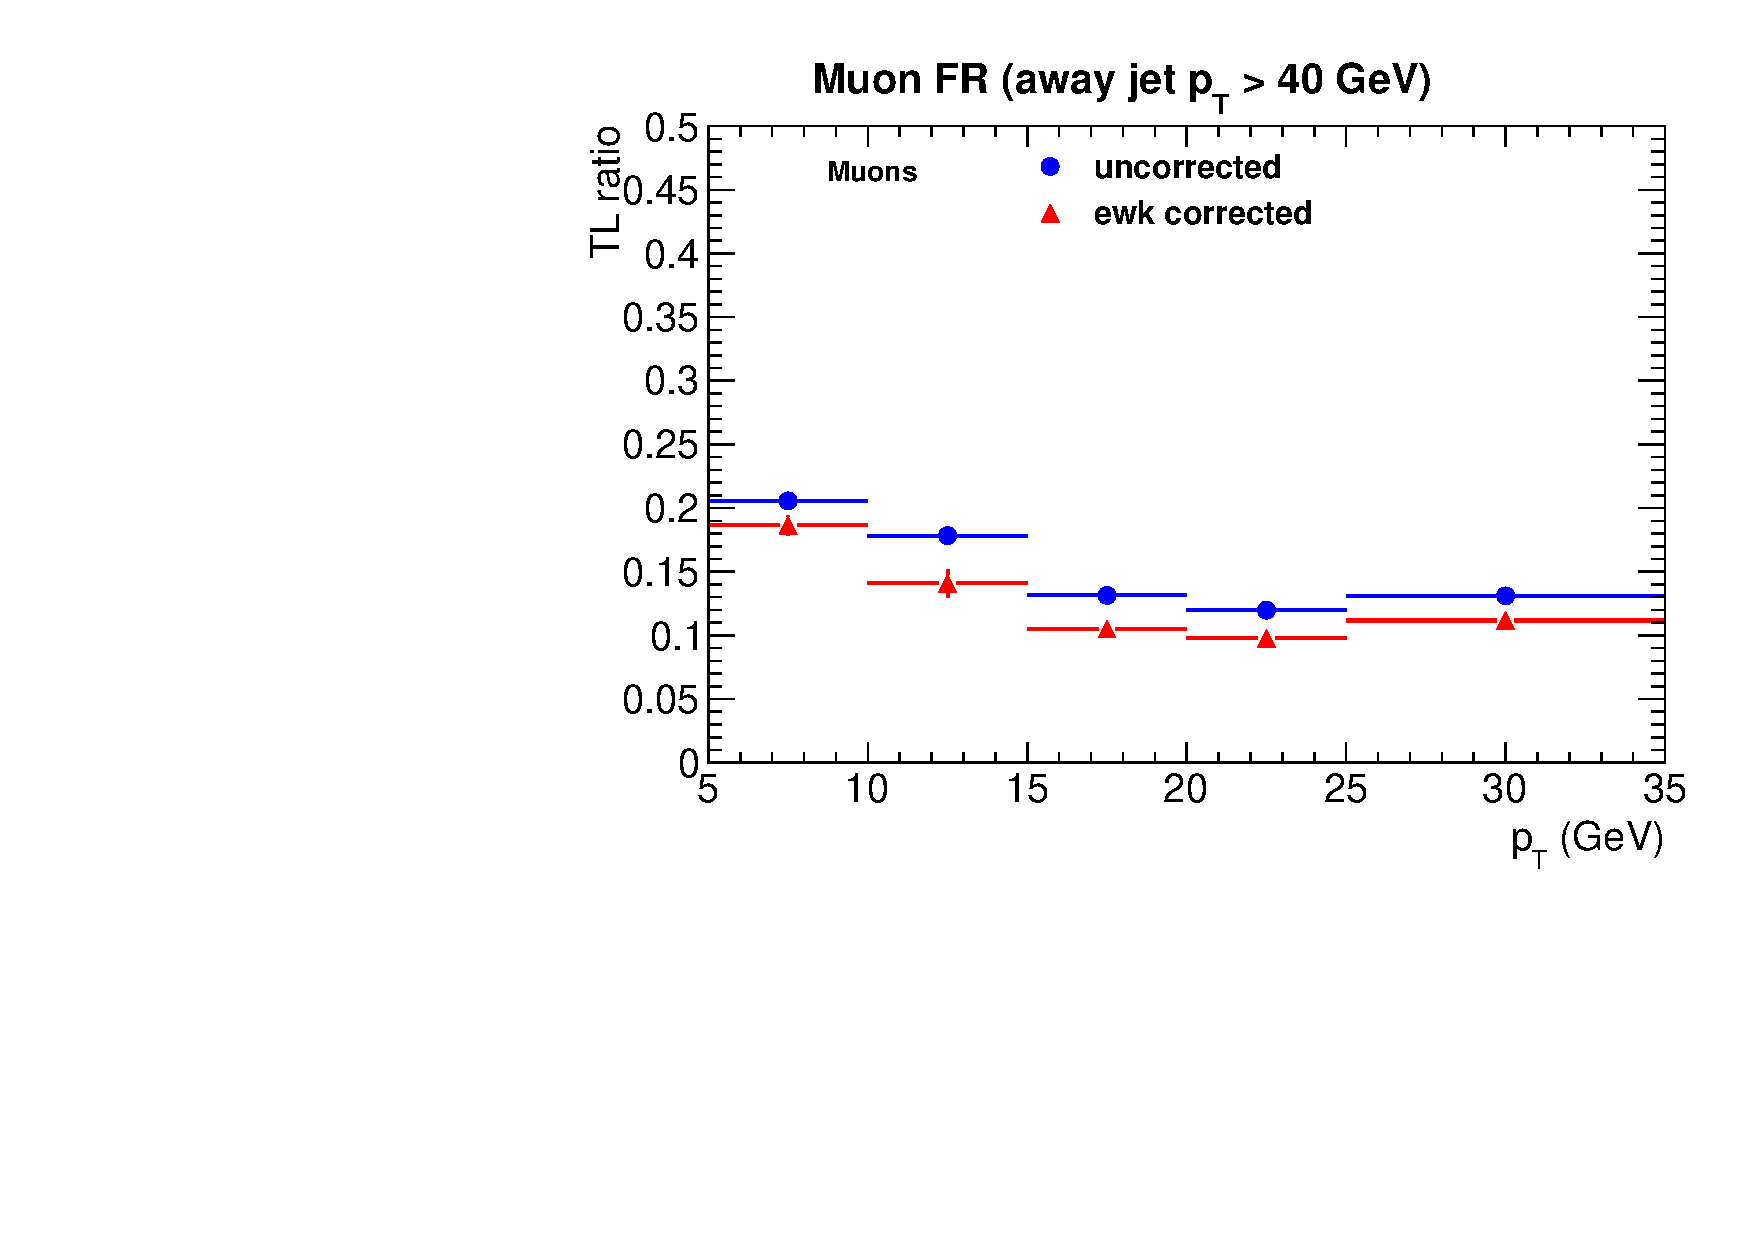
\includegraphics[width=0.48\textwidth]{p_mufr40c_vs_pt_compare_ewkcor}
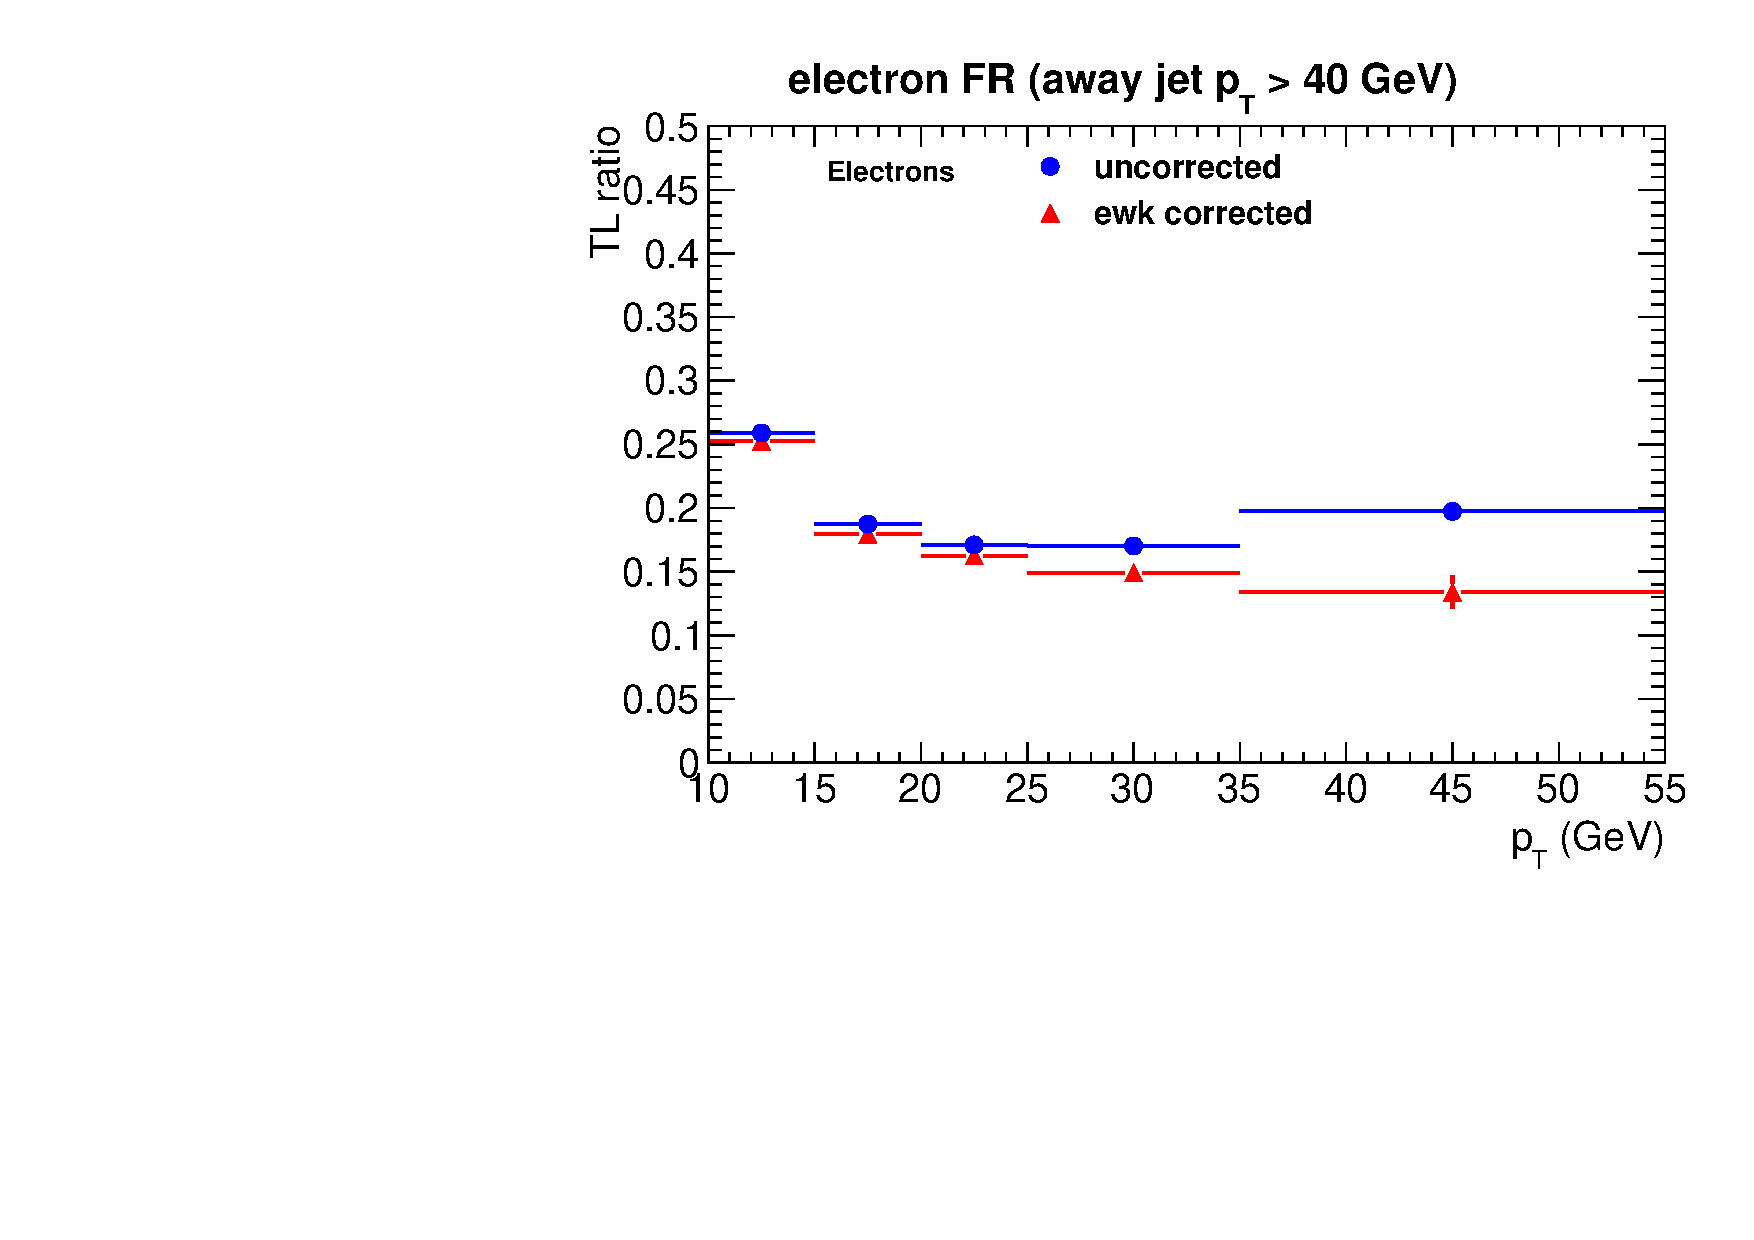
\includegraphics[width=0.48\textwidth]{p_elfr40c_vs_pt_compare_ewkcor}
\caption[The measured fake rate vs \pt before and after the electroweak corrections]
{\label{fig:bkgd_fakes_fr_mufr_ewkcont}
Projection of the muon (left) and electron (right) fake rate in data vs \pt.
The blue plot is the fake rate before the EWK correction and the red plot is
after.
}
\end{center}
\end{figure}
% --------------------------------------------------------------------------- %

% --------------------------------------------------------------------------- %
\subsection{Fake Rates for Electrons and Muons}
\label {sec:bkgd_fakes_fr}
% --------------------------------------------------------------------------- %
The fake rate is measured using the selections described
in Section~\ref{sec:bkgd_fakes_method}. As discussed in
Section~\ref{sec:bkgd_fakes_datasets}, the electron fake rates are
measured separately for the triggers with and without an online
isolation requirement. The results of the measurement for electrons are
summarized in Tables~\ref{tab:fr_elfr_hpt} and~\ref{tab:fr_elfr_lpt}.
The muon fake rates are measured using the single-muon triggers described
in Section~\ref{sec:bkgd_fakes_datasets}. The results are summarized in
Table~\ref{tab:fr_mufr}.

Figure~\ref{fig:bkgd_fakes_fr_mufr} shows the \pt, \aeta, and \nvtx projections
of the fake rate as measured in data. The fake rate is approximately flat in
\aeta. The FR decreases with increasing \pt, from a value of approximately 0.2
at 5 \GeV to about 0.13 at \hpt. The highest \pt bin shows a slight increase
in the fake rate that may be an indication that \W contamination is present,
but the increase is not significant enough to warrant considerable attentions
at this point. We assume that the fake rate is mostly constant above a $\pt >
35~\GeV$ so we assume this value in the last bin for all leptons greater than 35
\GeV.

Figure~\ref{fig:bkgd_fakes_fr_elfr} shows the \pt, \aeta, and \nvtx projections
for the electron fake rate measured with and without an online isolation
requirement. The fake rate is relatively stable, although it does show a slight
upward trend at \hpt. This is more pronounced in the fake rate with the online
isolation. Overall, the fake rate without the isolation requirement is higher
than with it, which is expected since this allows more non-prompt leptons to be
considered (due to higher denominator lepton counts). We assume that the fake
rate is mostly constant above a $\pt > 55~\GeV$ so we assume this value in the
last bin for all leptons greater than 55 \GeV.
% --------------------------------------------------------------------------- %
\begin{figure}[!hbt]
\begin{center}
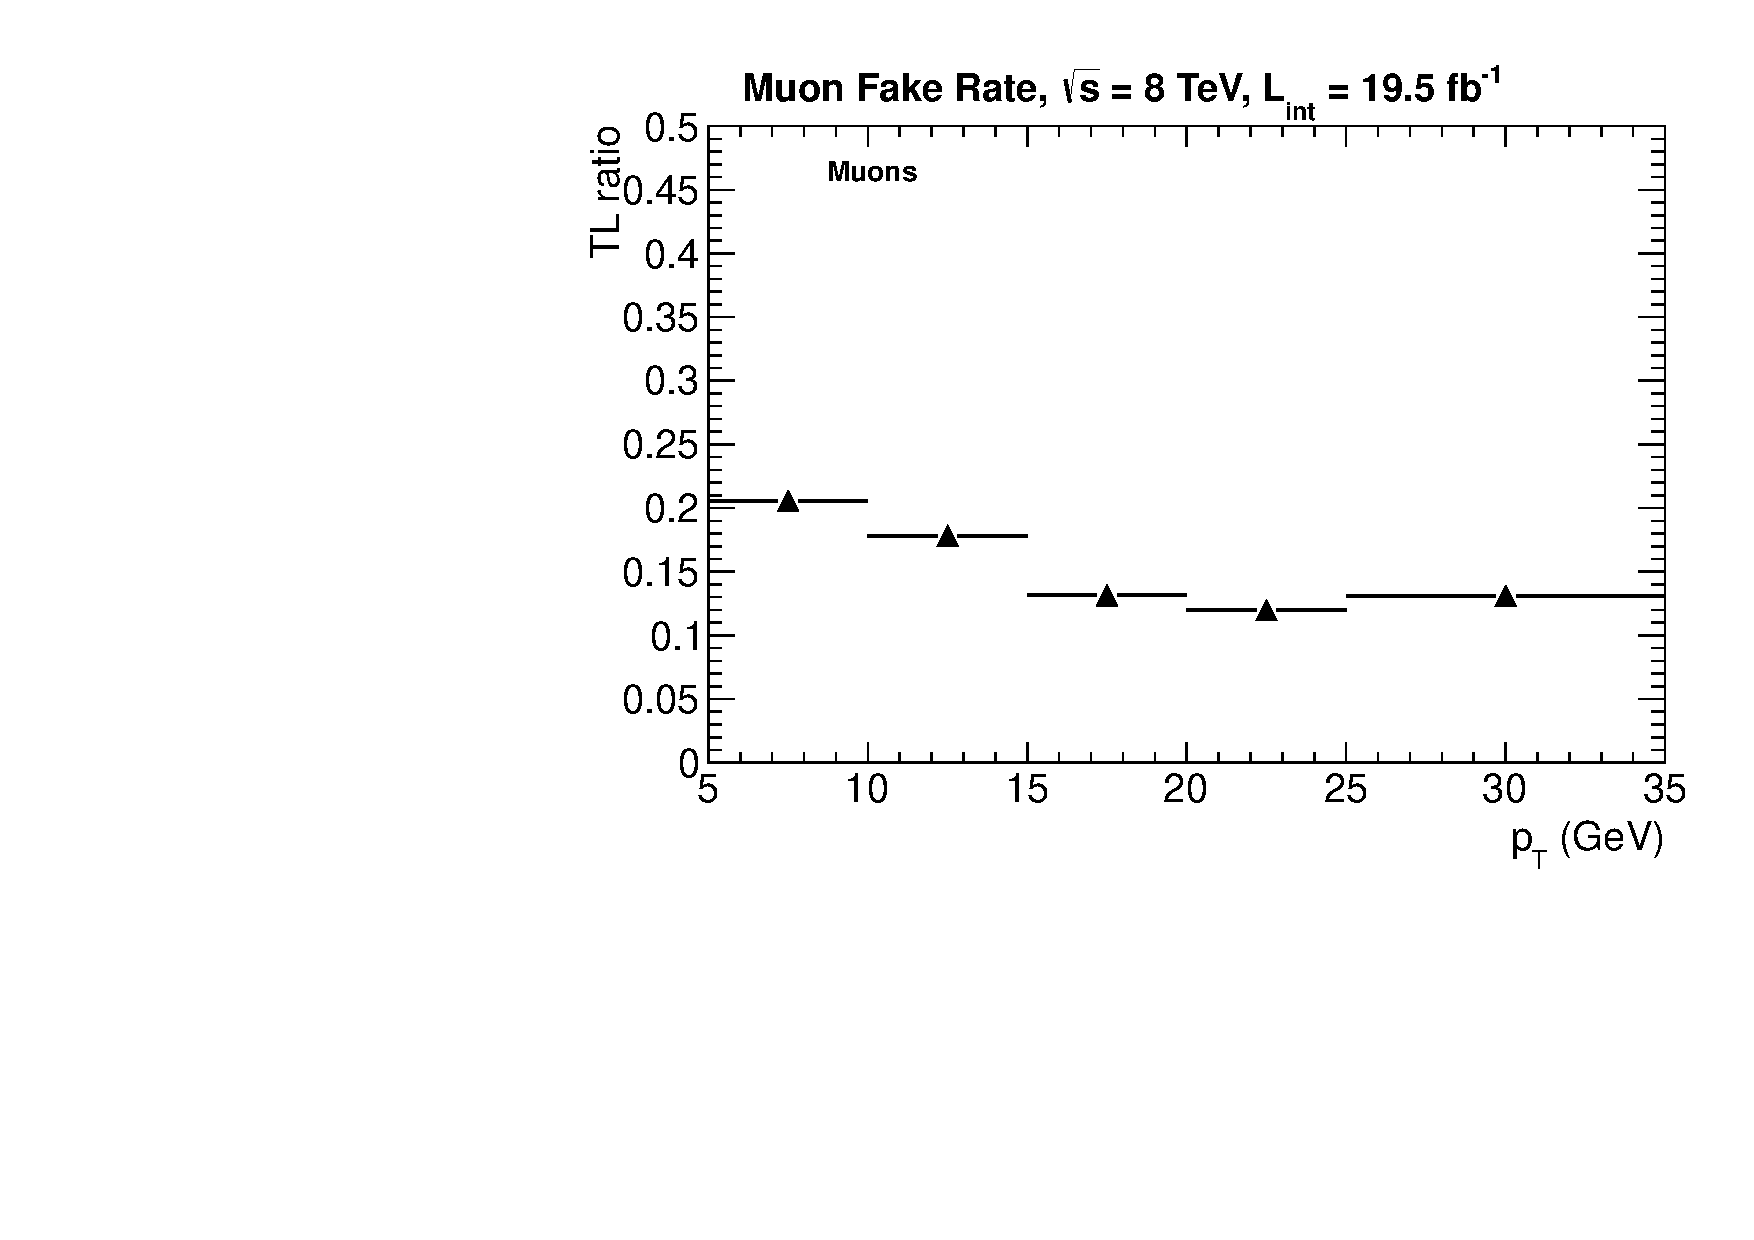
\includegraphics[width=0.48\textwidth]{p_mufr_aj40_vs_pt}
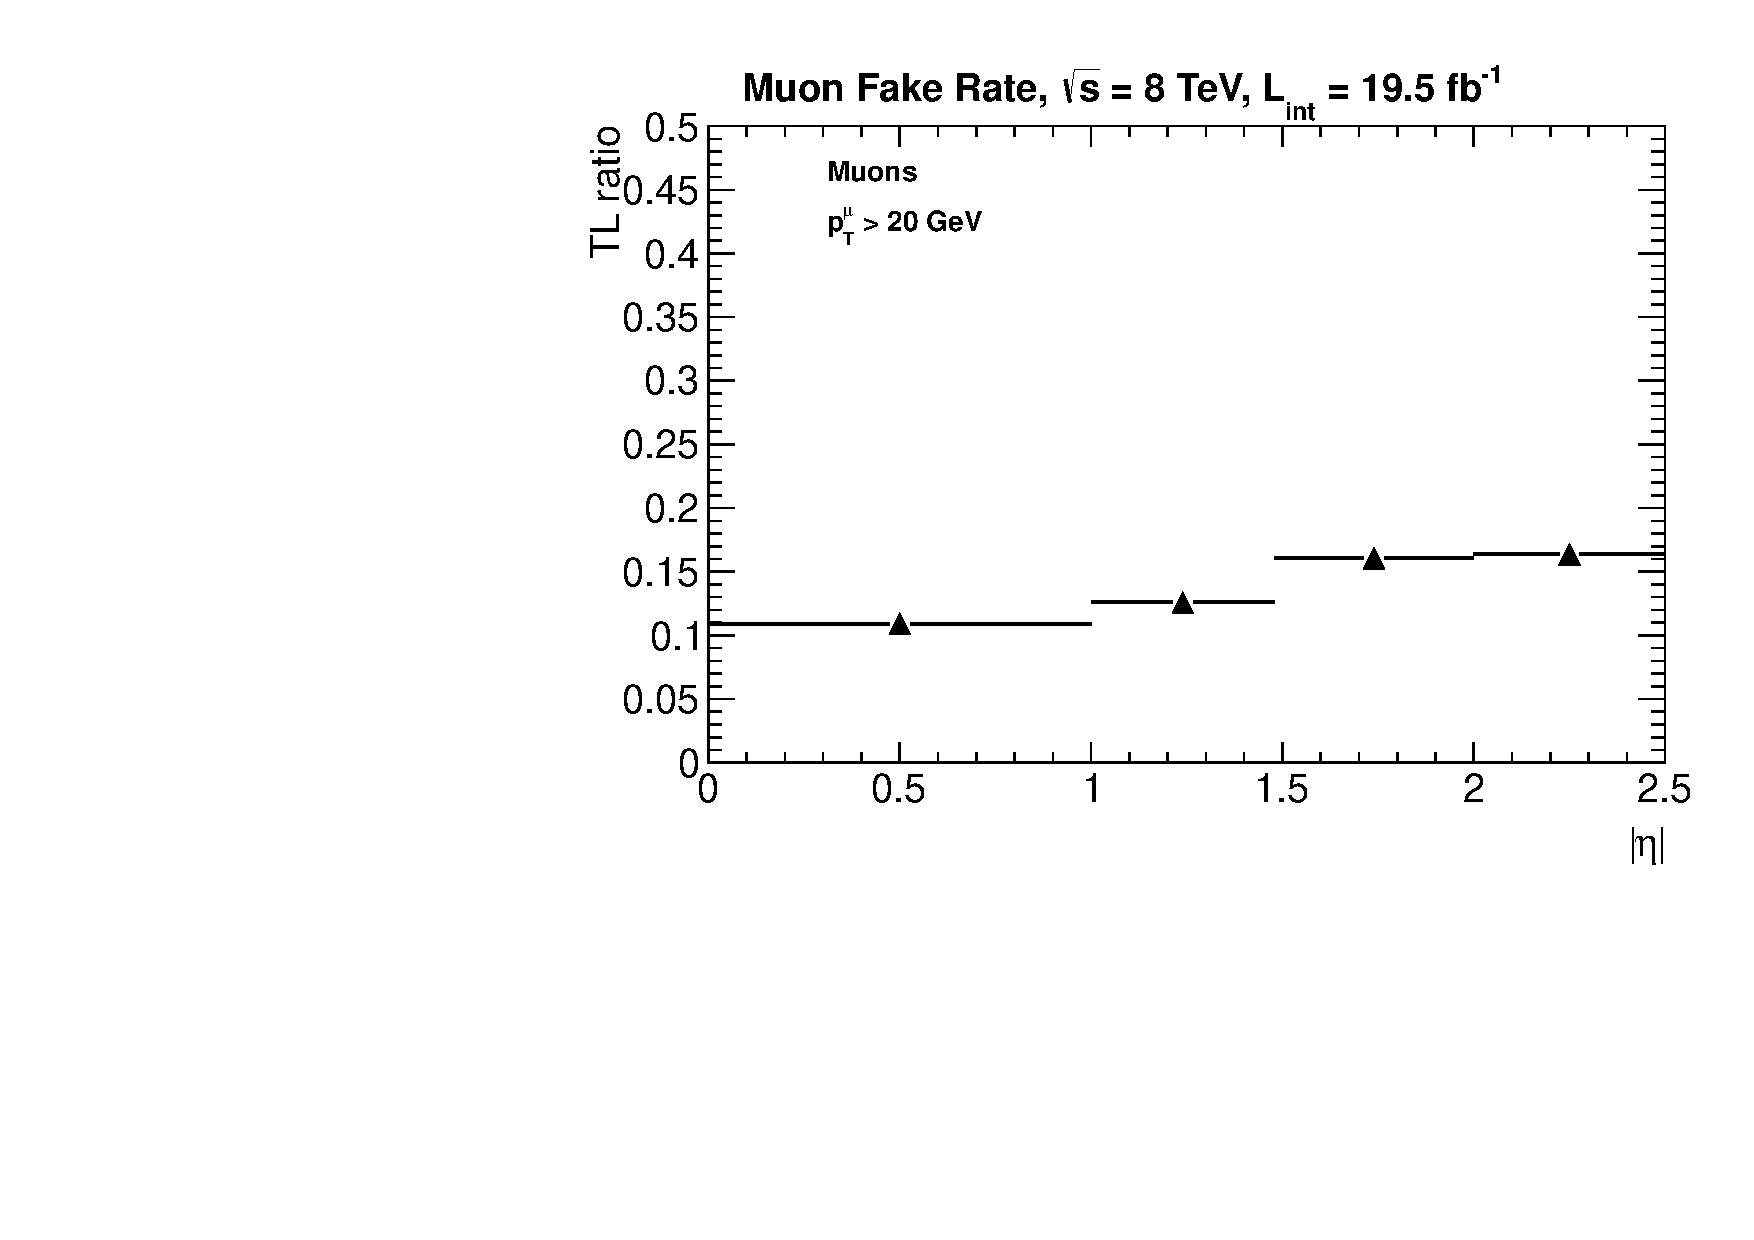
\includegraphics[width=0.48\textwidth]{p_mufr_aj40_vs_eta}
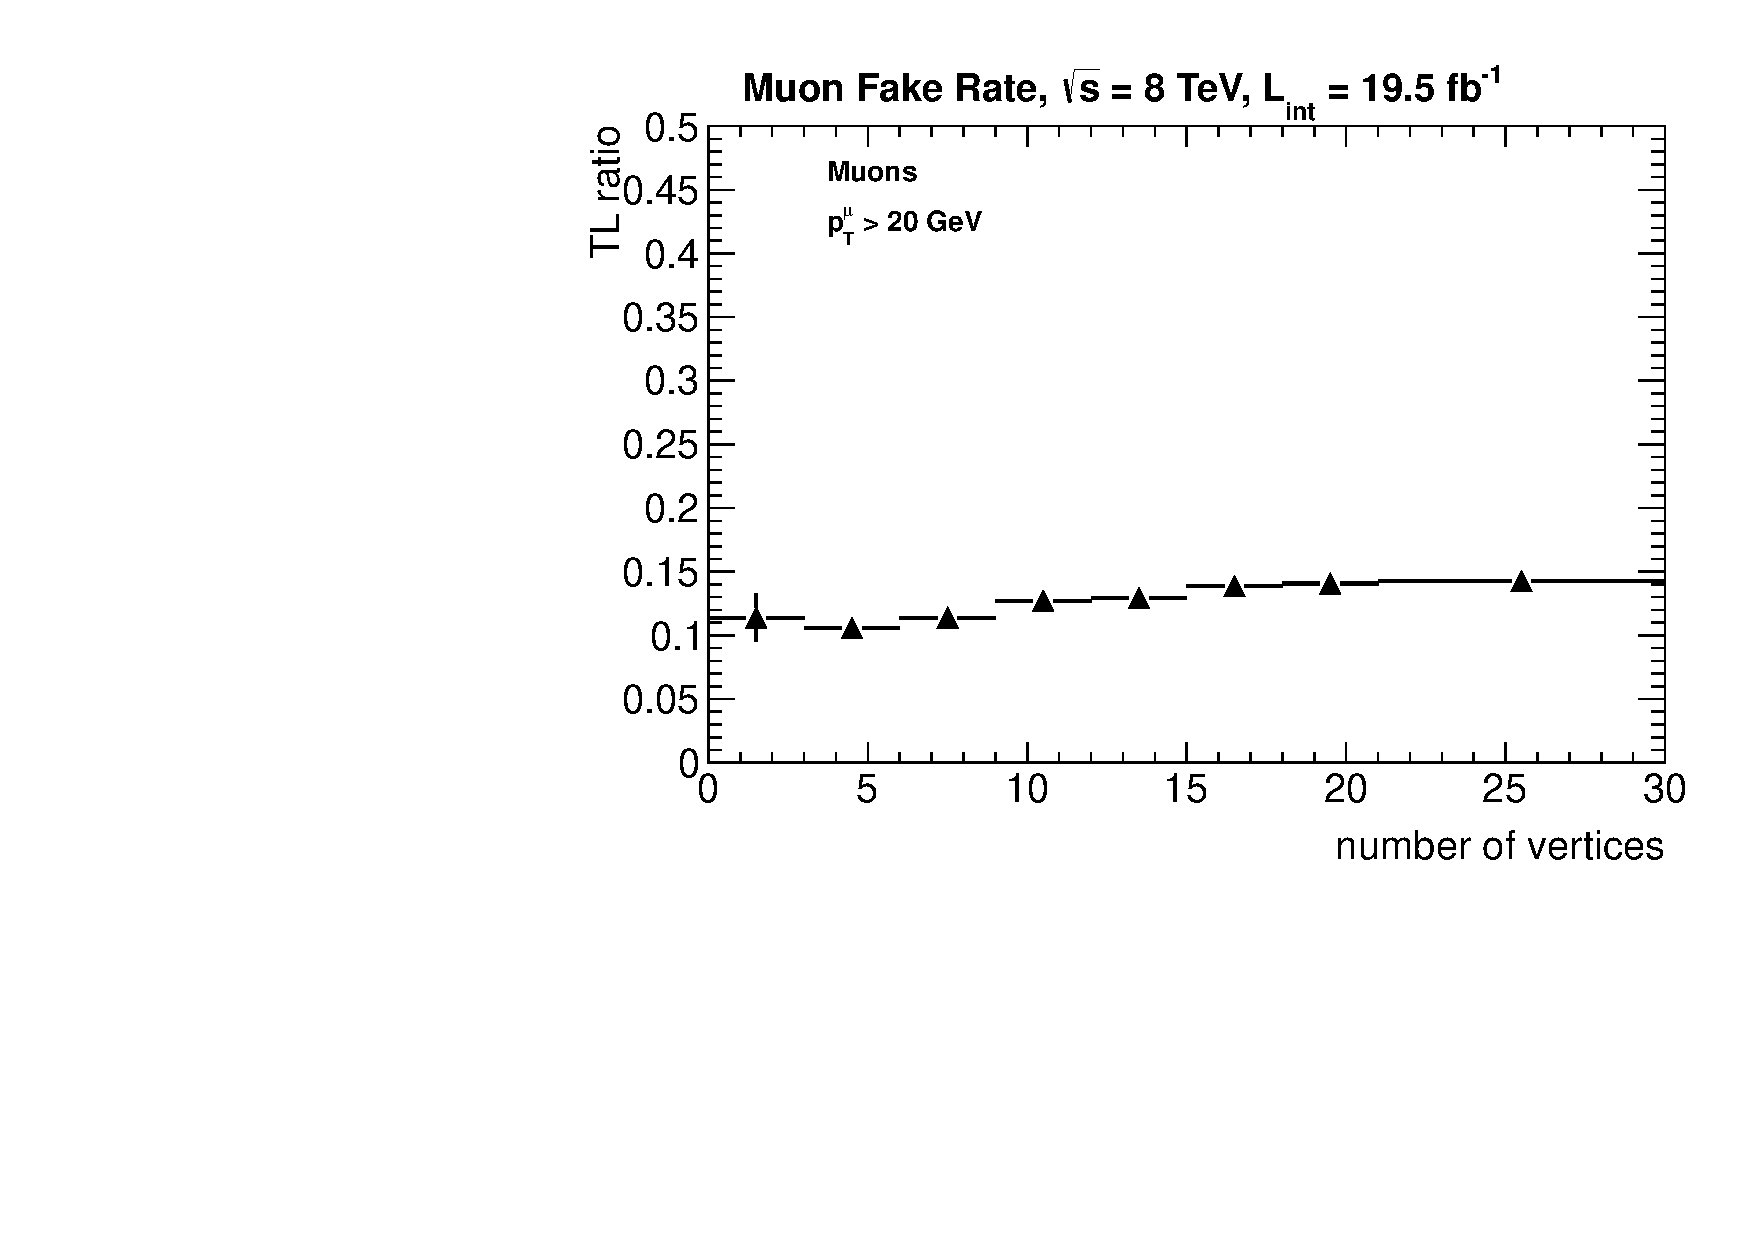
\includegraphics[width=0.48\textwidth]{p_mufr_aj40_vs_nvtxs}
\caption[Muon Fake Rate vs \pt, \aeta, and number of vertices]
{\label{fig:bkgd_fakes_fr_mufr_aj}
Projection of the muon fake rate in data vs \aeta, \pt, and the number of
vertices. This fake rate is use for both the \hpt and \lpt analysis.
}
\end{center}
\end{figure}
% --------------------------------------------------------------------------- %

% --------------------------------------------------------------------------- %
\begin{figure}[!hbt]
\begin{center}
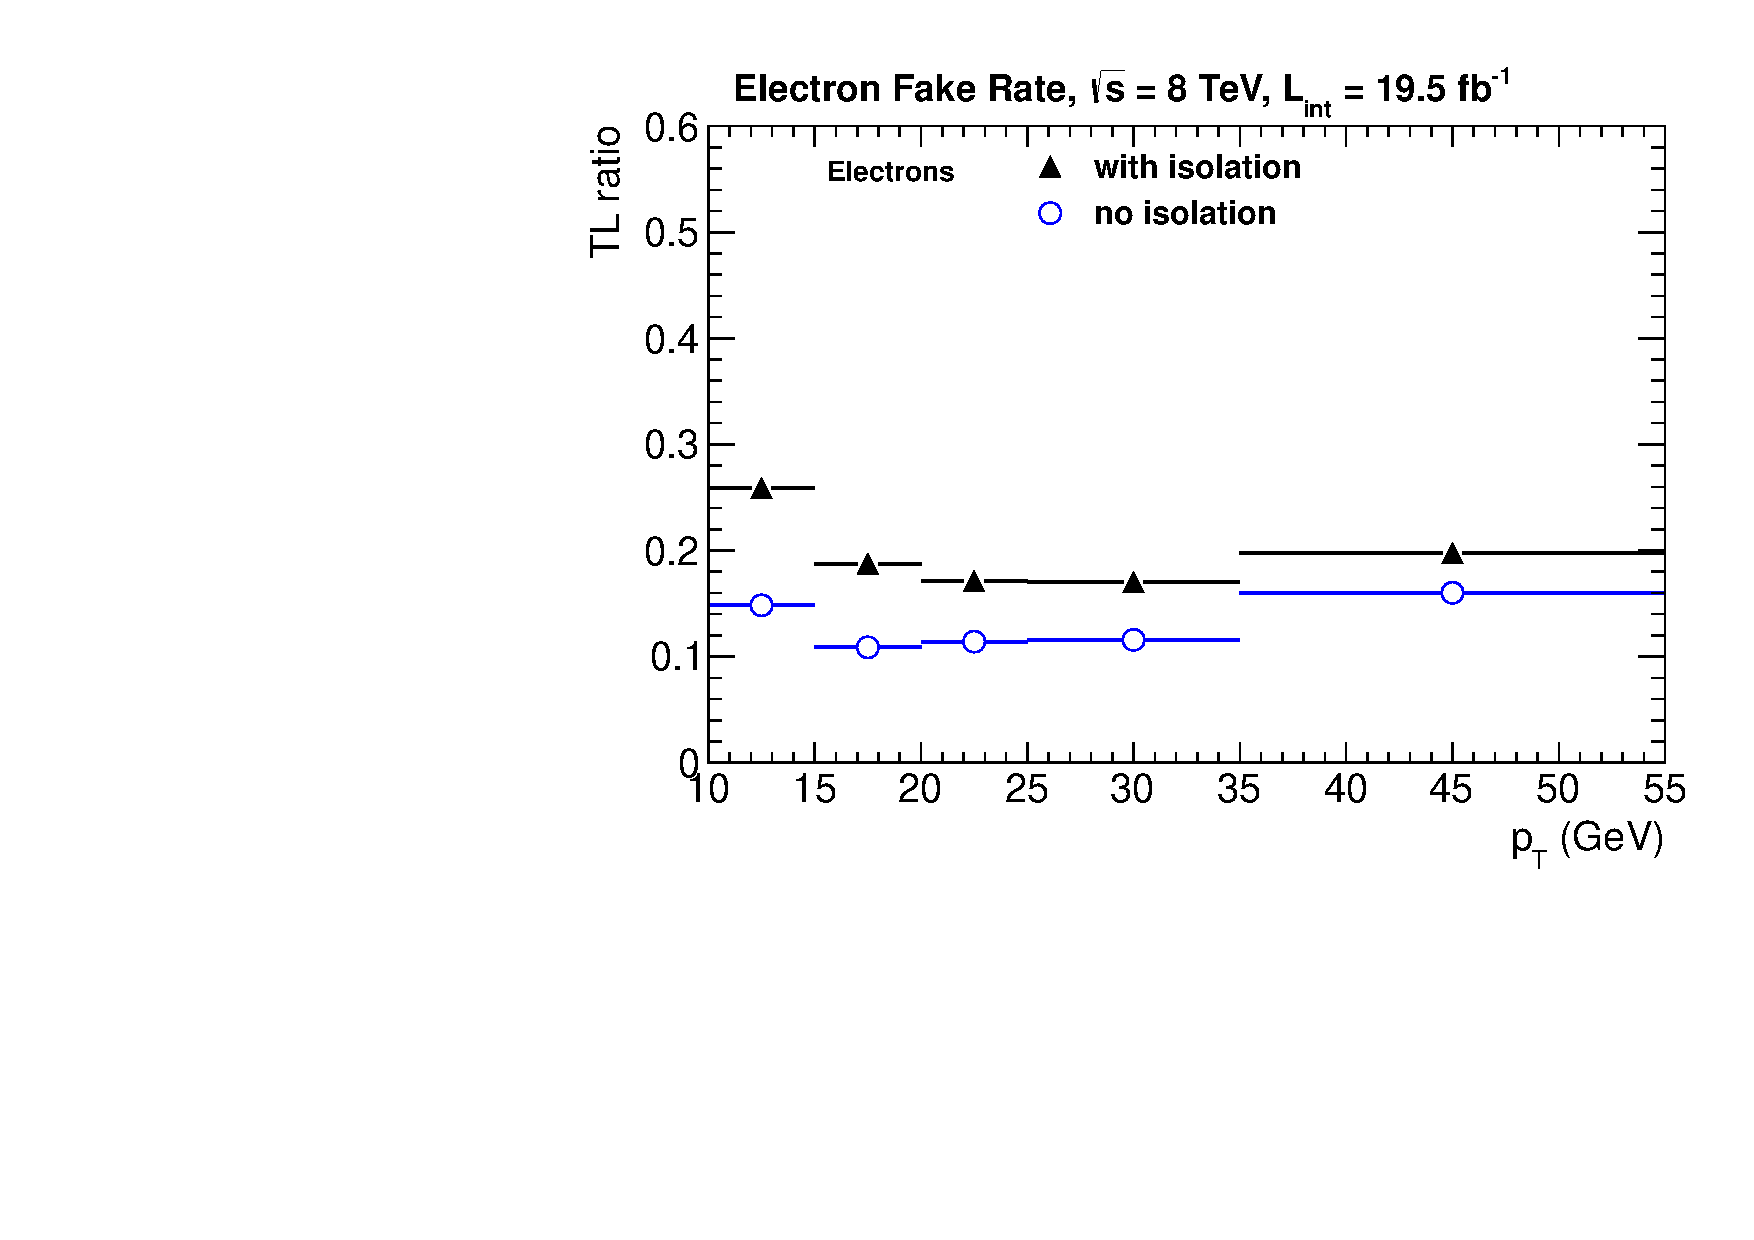
\includegraphics[width=0.48\textwidth]{p_elfr_aj40_vs_pt}
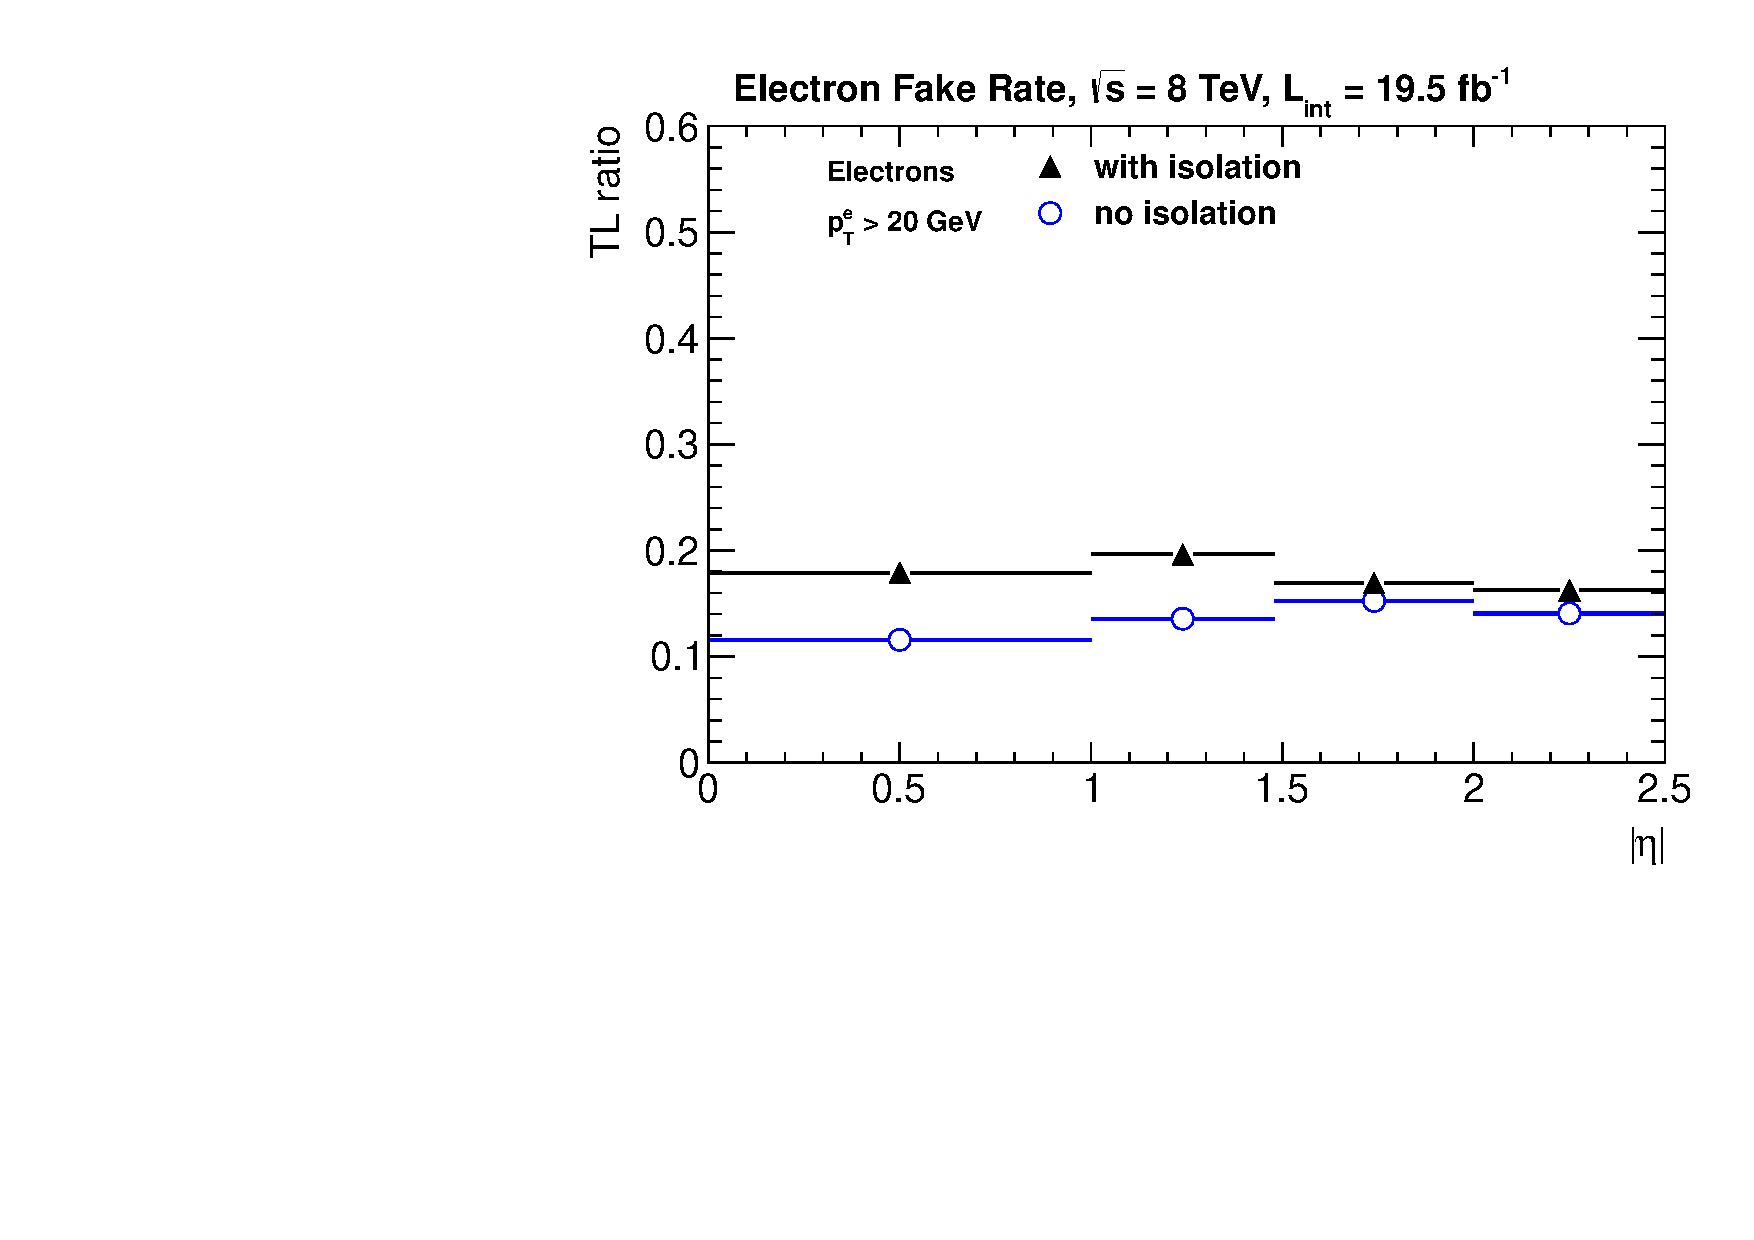
\includegraphics[width=0.48\textwidth]{p_elfr_aj40_vs_eta}
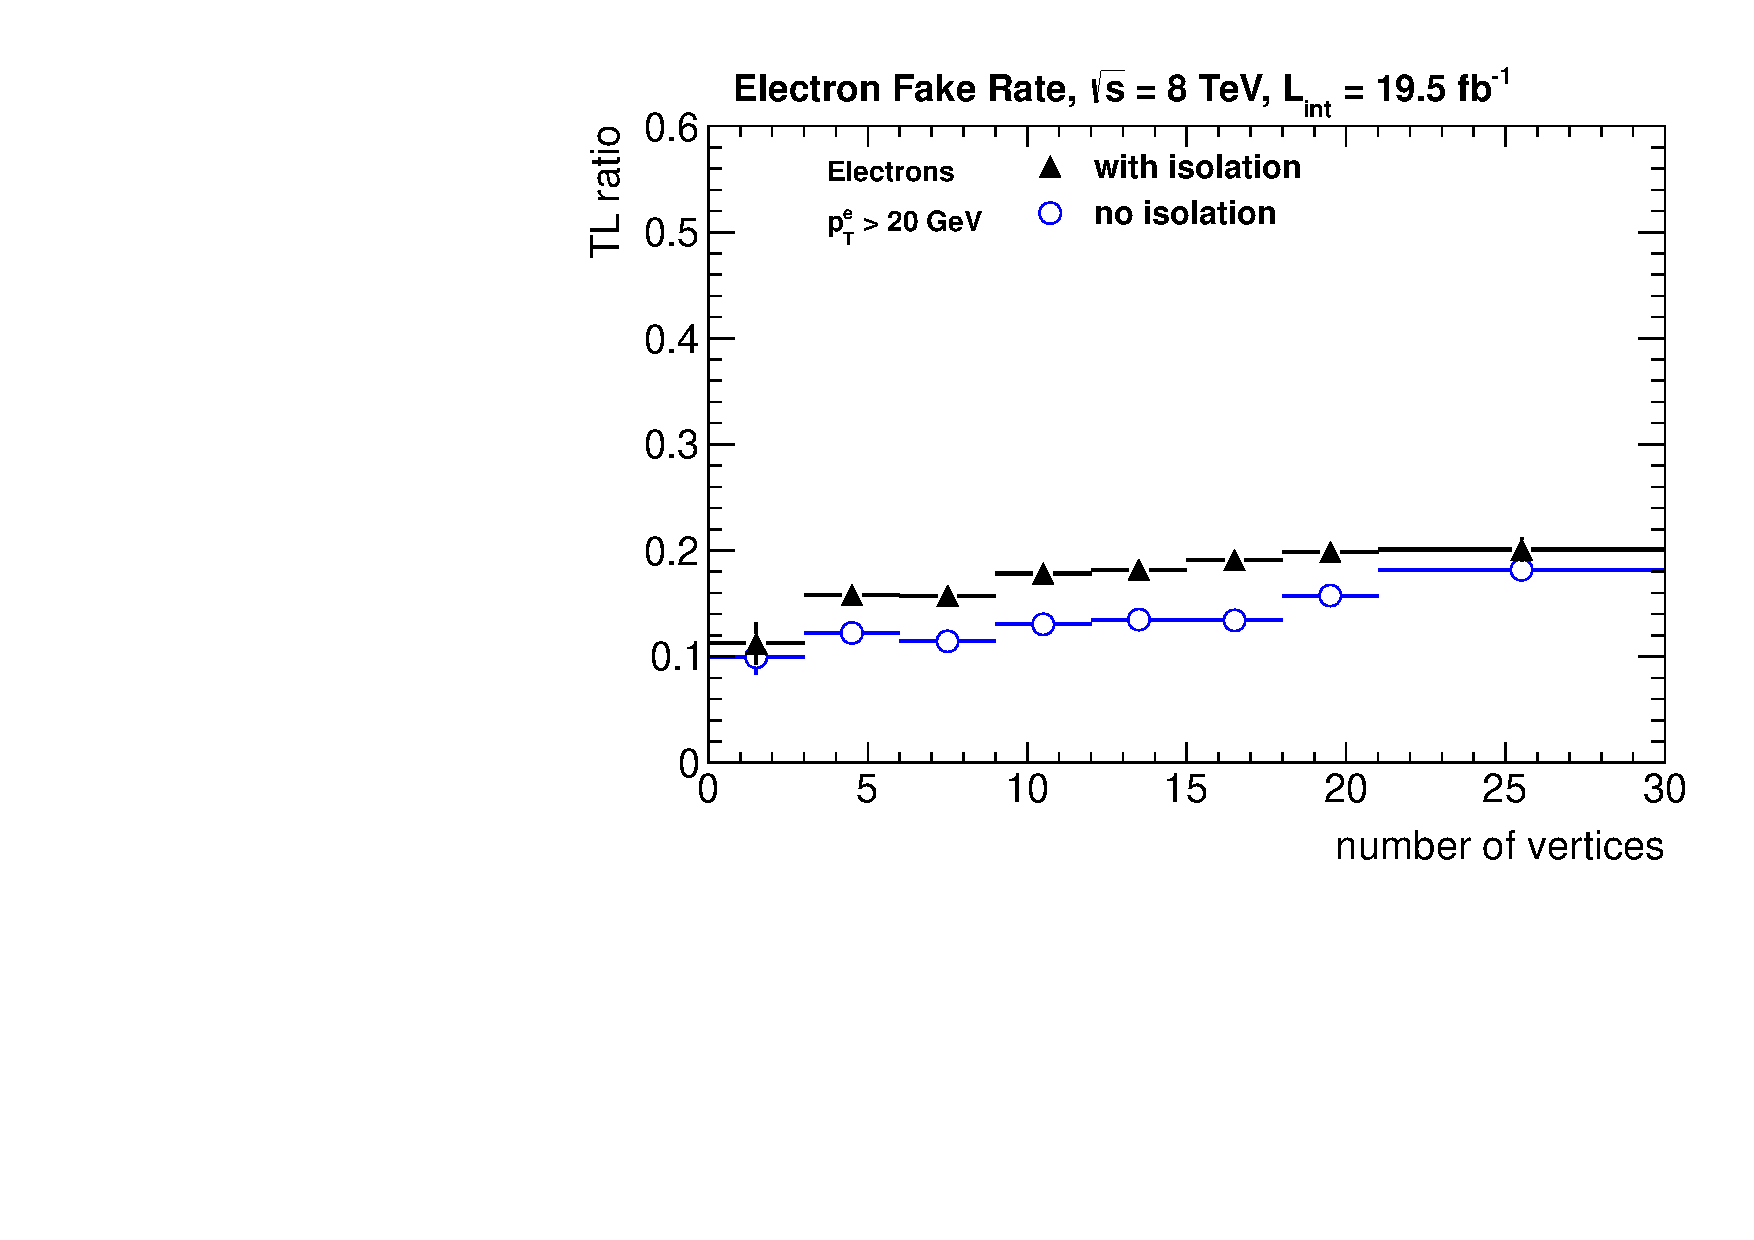
\includegraphics[width=0.48\textwidth]{p_elfr_aj40_vs_nvtxs}
\caption[Electron Fake Rate vs \pt, \aeta, and number of vertices]
{\label{fig:bkgd_fakes_fr_elfr_aj}
Projection of the electron fake rate in data vs \aeta, \pt, and the number
of vertices with (triangles) and without (open circles) an online isolation
requirement. The fake rate measured with an online isolation requirement
is used for the \hpt analysis. The triggers without the online isolation
requirement are used in the fake rate for the \lpt analysis.
}
\end{center}
\end{figure}
% --------------------------------------------------------------------------- %
% 
% --------------------------------------------------------------------------- %
\subsection{Study of Fake Rate Dependencies}
\label {sec:bkgd_fakes_frstudy}
% --------------------------------------------------------------------------- %
Several studies are performed in data and simulation to assess the dependence
of the fake rate on the kinematics. Studies of the contaminations of
the fake rate in data due to prompt leptons was already considered in
Section~\ref{sec:bkgd_fakes_lepcont}. Here we perform the following two
studies:
\begin{itemize}
\item Measurement of the fake rate dependence on the away-side jet \pt, as a
measure of the dependence of the parent parton momentum.
\item Closure test are performed using simulated QCD, \Wj, and \ttbar samples.
\end{itemize}

% --------------------------------------------------------------------------- %
\subsubsection{Fake Rate Dependence on Away Jet \pt}
\label {sec:bkgd_fakes_frstudy_aj}
% --------------------------------------------------------------------------- %
The lepton fake rates are dependent upon the away-jet requirement because
of the extrapolation in isolation. Lepton candidates in \hpt jets have a
smaller probability to pass an isolation requirement than a similar \pt lepton
candidate in a \lpt jet. The difference can be understood by considering the
relative size of the lepton \pt and the difference between the parent parton's
\pt with the lepton's \pt ($|\pt^{parton} - \pt^{lepton}|$). The latter is a
measure of the maximum transverse energy that can be deposited in the isolation
cone. Thus, for a given lepton \pt, the higher the \pt of the originating
parton, the less likely it is for this lepton to pass the numerator isolation
criteria. The probability levels off when the momentum of the parton because
much larger than that of the lepton candidate.

Figures~\ref{fig:bkgd_fakes_fr_mufr}-\ref{fig:bkgd_fakes_fr_elfr_noiso} show
the \aeta and \pt projections for the muon and electron fake rates measured in
the data with \pt $>20$, 40, and 60 \GeV away-jet requirements. The range of
jet \pt considered was determined by looking at the typical \pt spectrum of
\bqs with FO daughters in simulated \ttbar events. The dependence of the muon
fake rate on the away-jet \pt requirement is $\sim 30\%$. The dependence is
flat in \aeta, but increases with \pt for the muon candidate. The dependence of
the electron fake rates on the away-jet \pt is similarly $\sim 30\%$. There is
not a strong trend in either \aeta or \pt. The dependence appears similar for
electron fake rates measured with and without an isolation requirement.

% --------------------------------------------------------------------------- %
\begin{figure}[!hbt]
\begin{center}
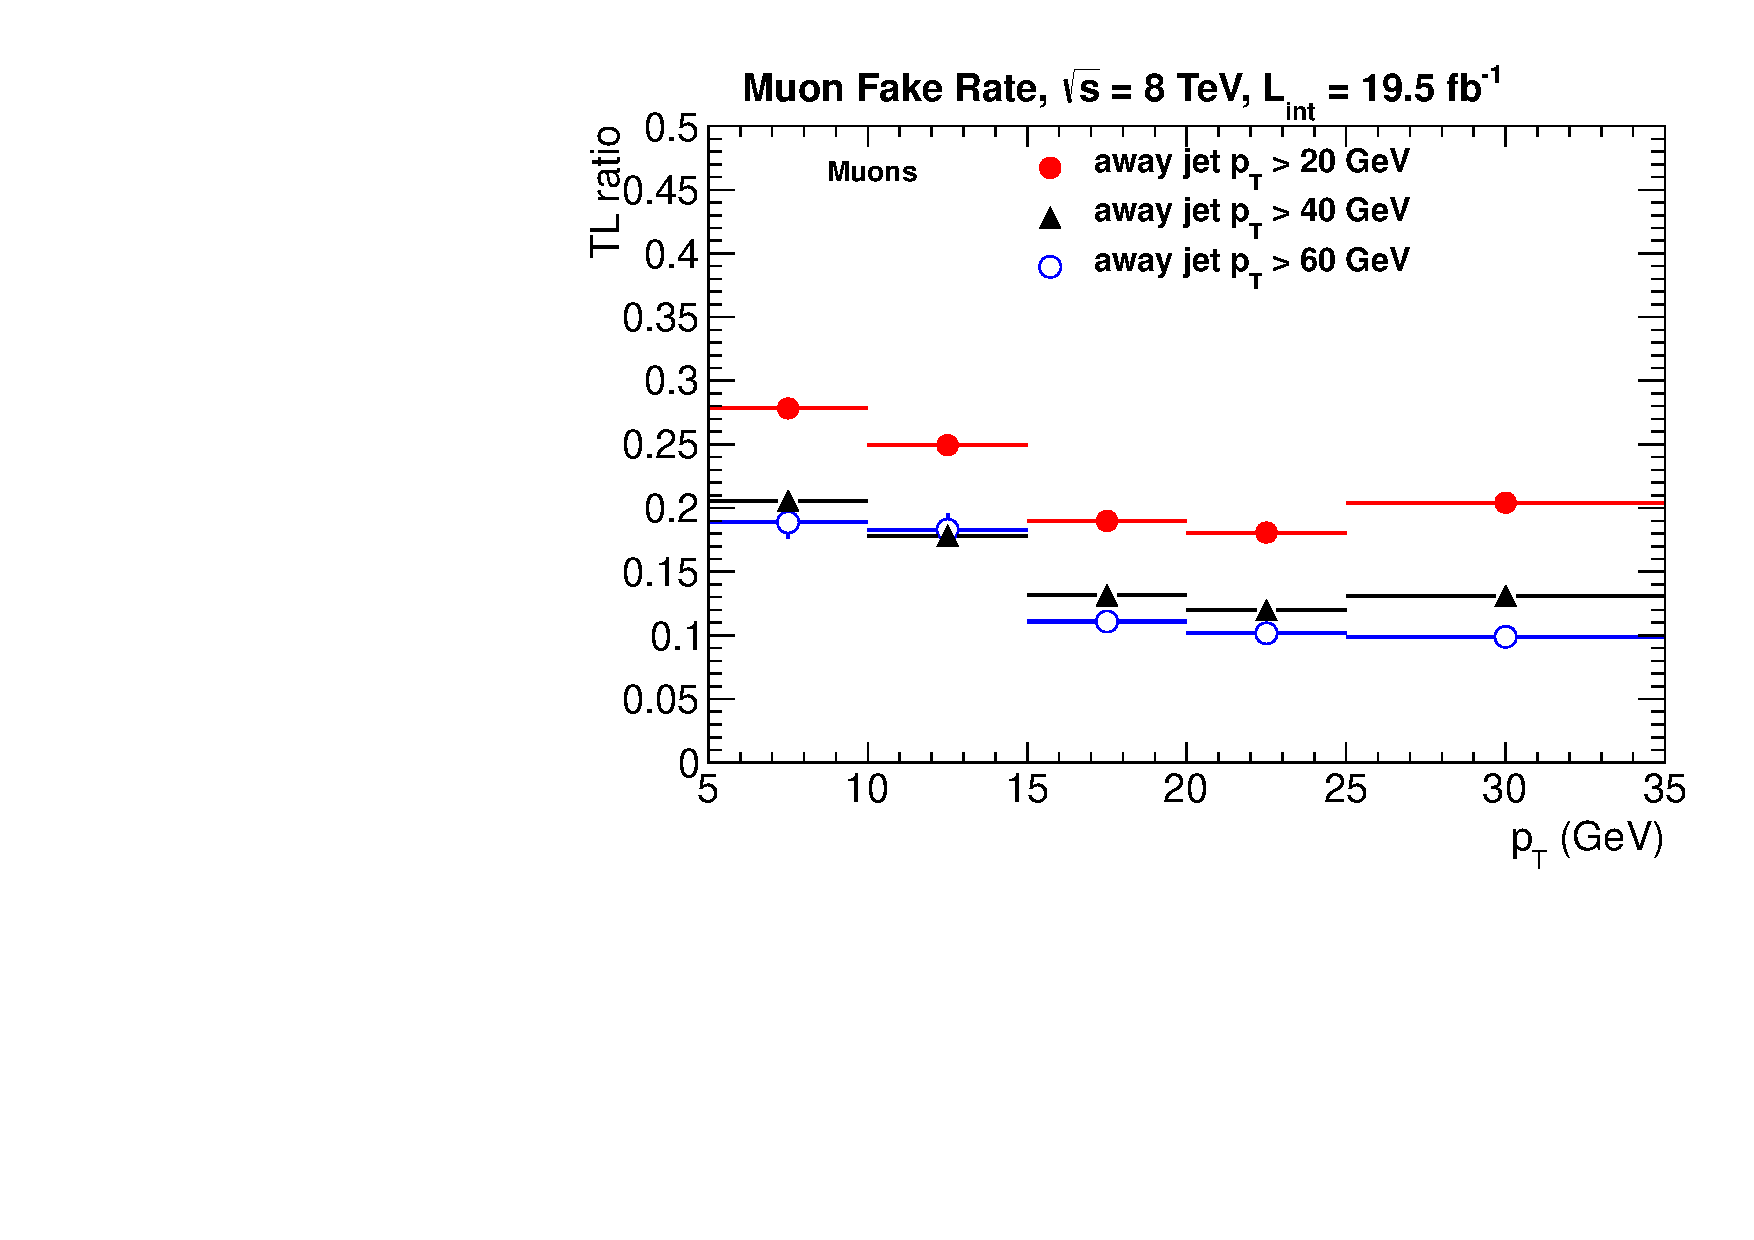
\includegraphics[width=0.48\textwidth]{p_mufr_vs_pt}
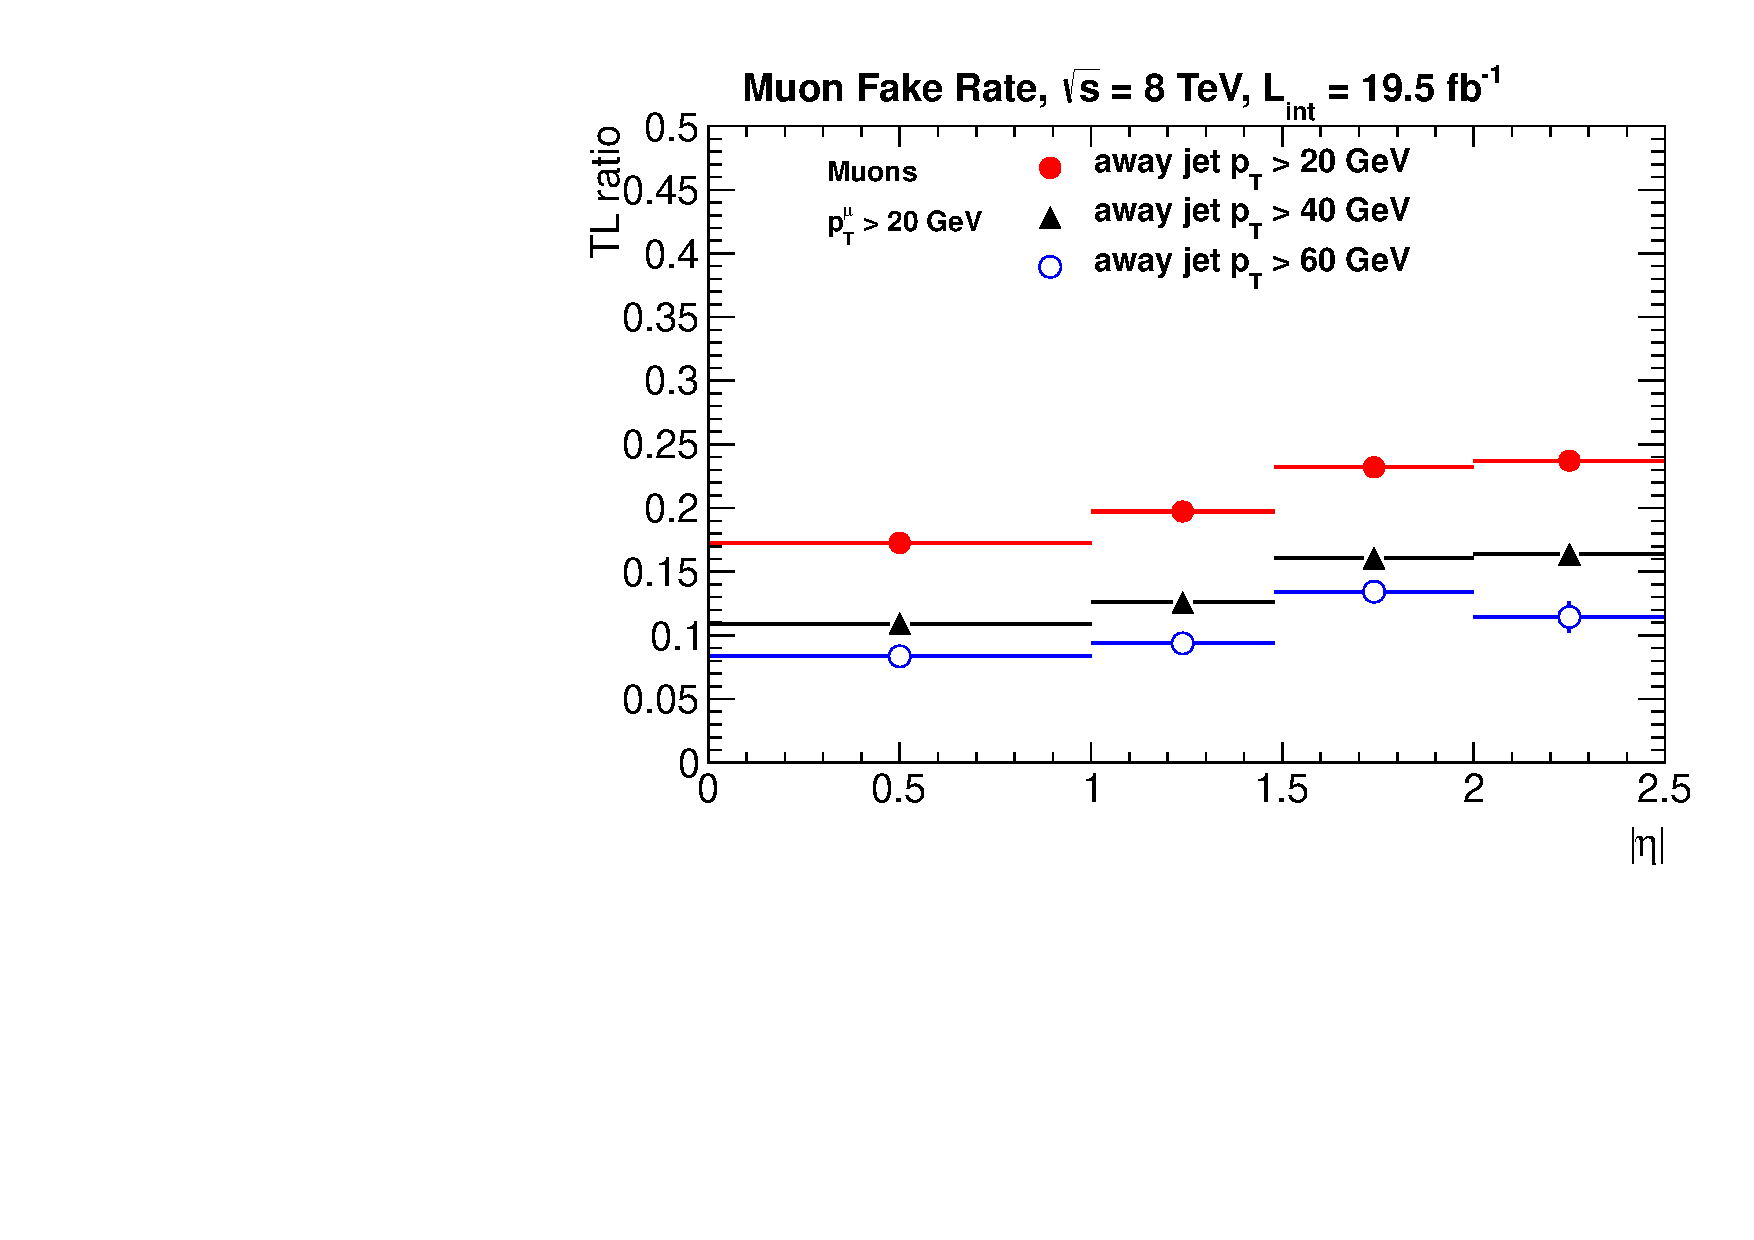
\includegraphics[width=0.48\textwidth]{p_mufr_vs_eta}
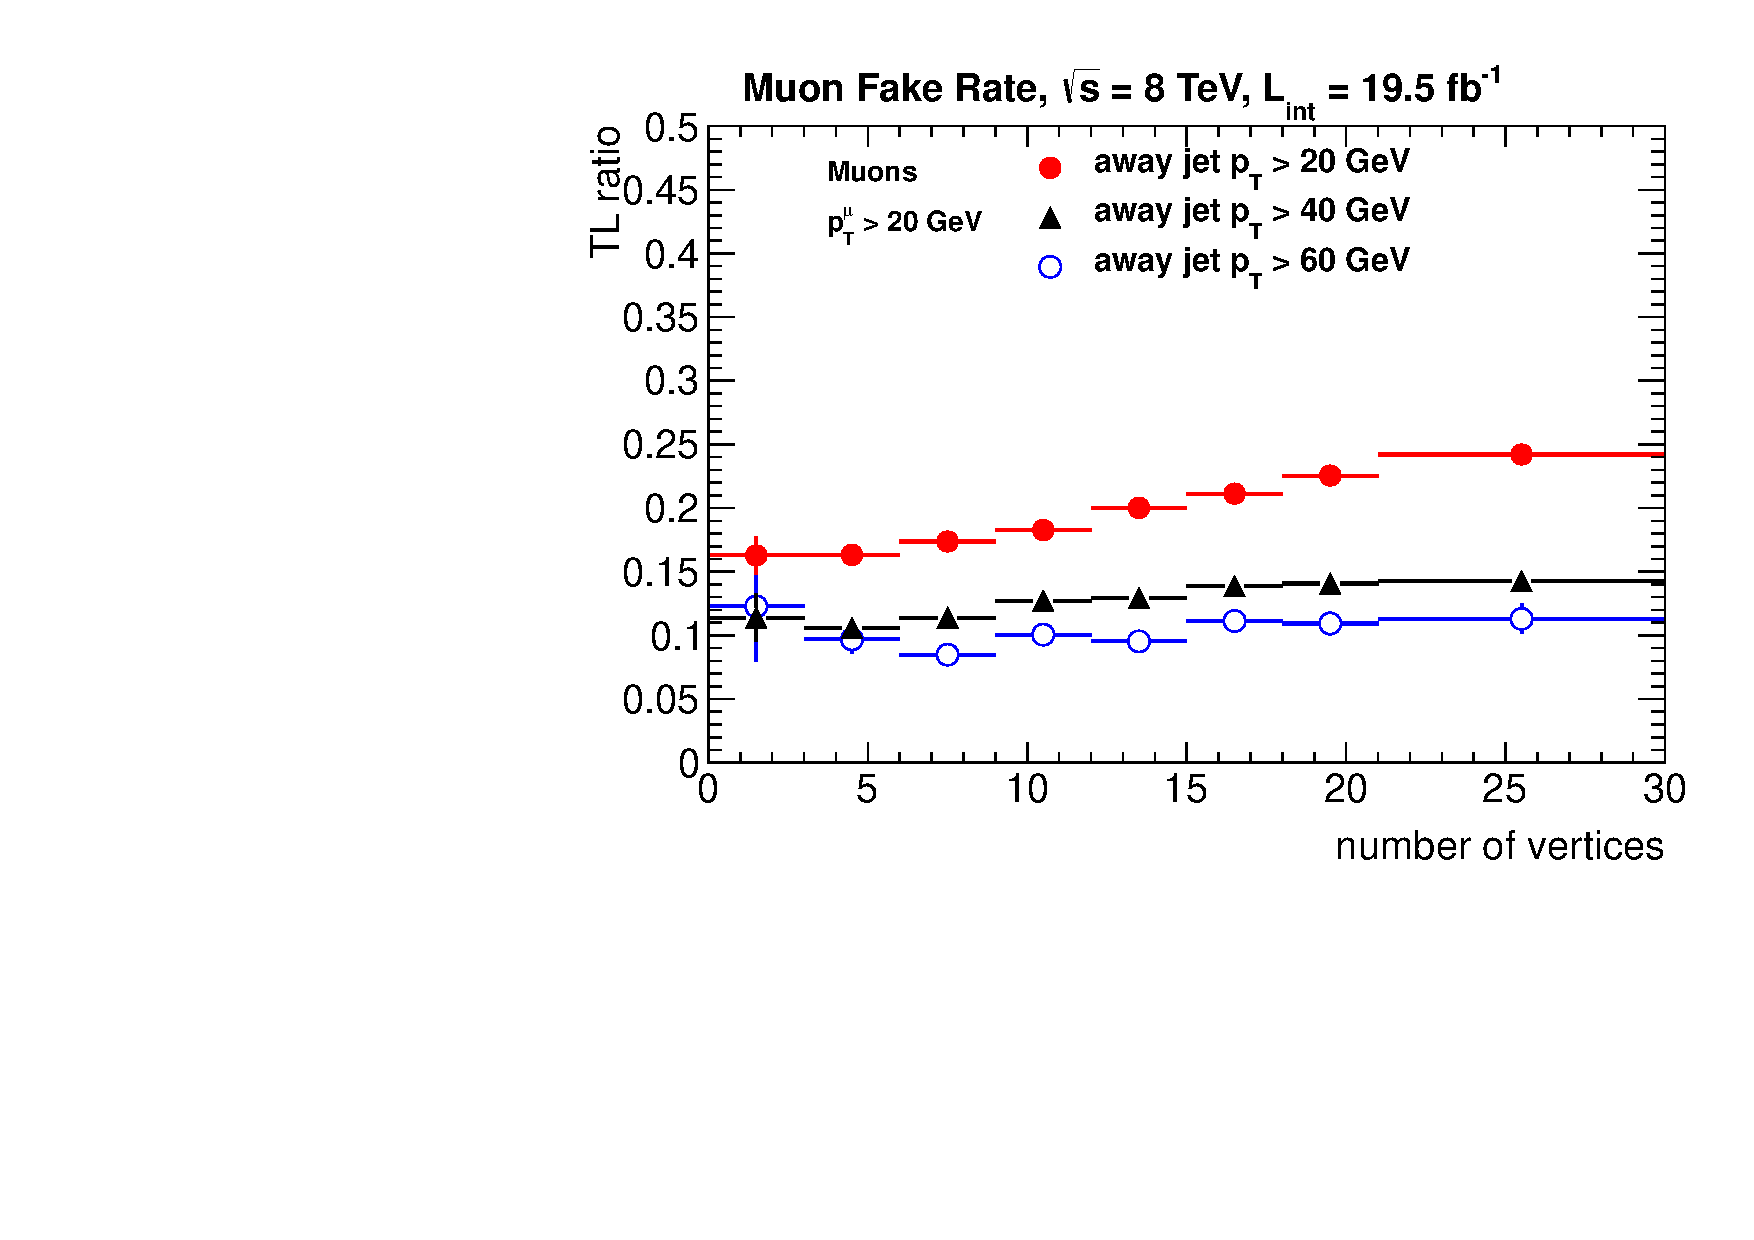
\includegraphics[width=0.48\textwidth]{p_mufr_vs_nvtxs}
\caption[Muon Fake Rate vs \pt, \aeta, and number of vertices for different away jet \pt requirements]
{\label{fig:bkgd_fakes_fr_mufr}
Projection of the muon fake rate in data vs \aeta, \pt, and \nvtx for different
away jet \pt requirements. The away jet is a corrected particle flow jet and is
required to be $\DR > 0.1$ away from the muon candidate.
}
\end{center}
\end{figure}
% --------------------------------------------------------------------------- %

% --------------------------------------------------------------------------- %
\begin{figure}[!hbt]
\begin{center}
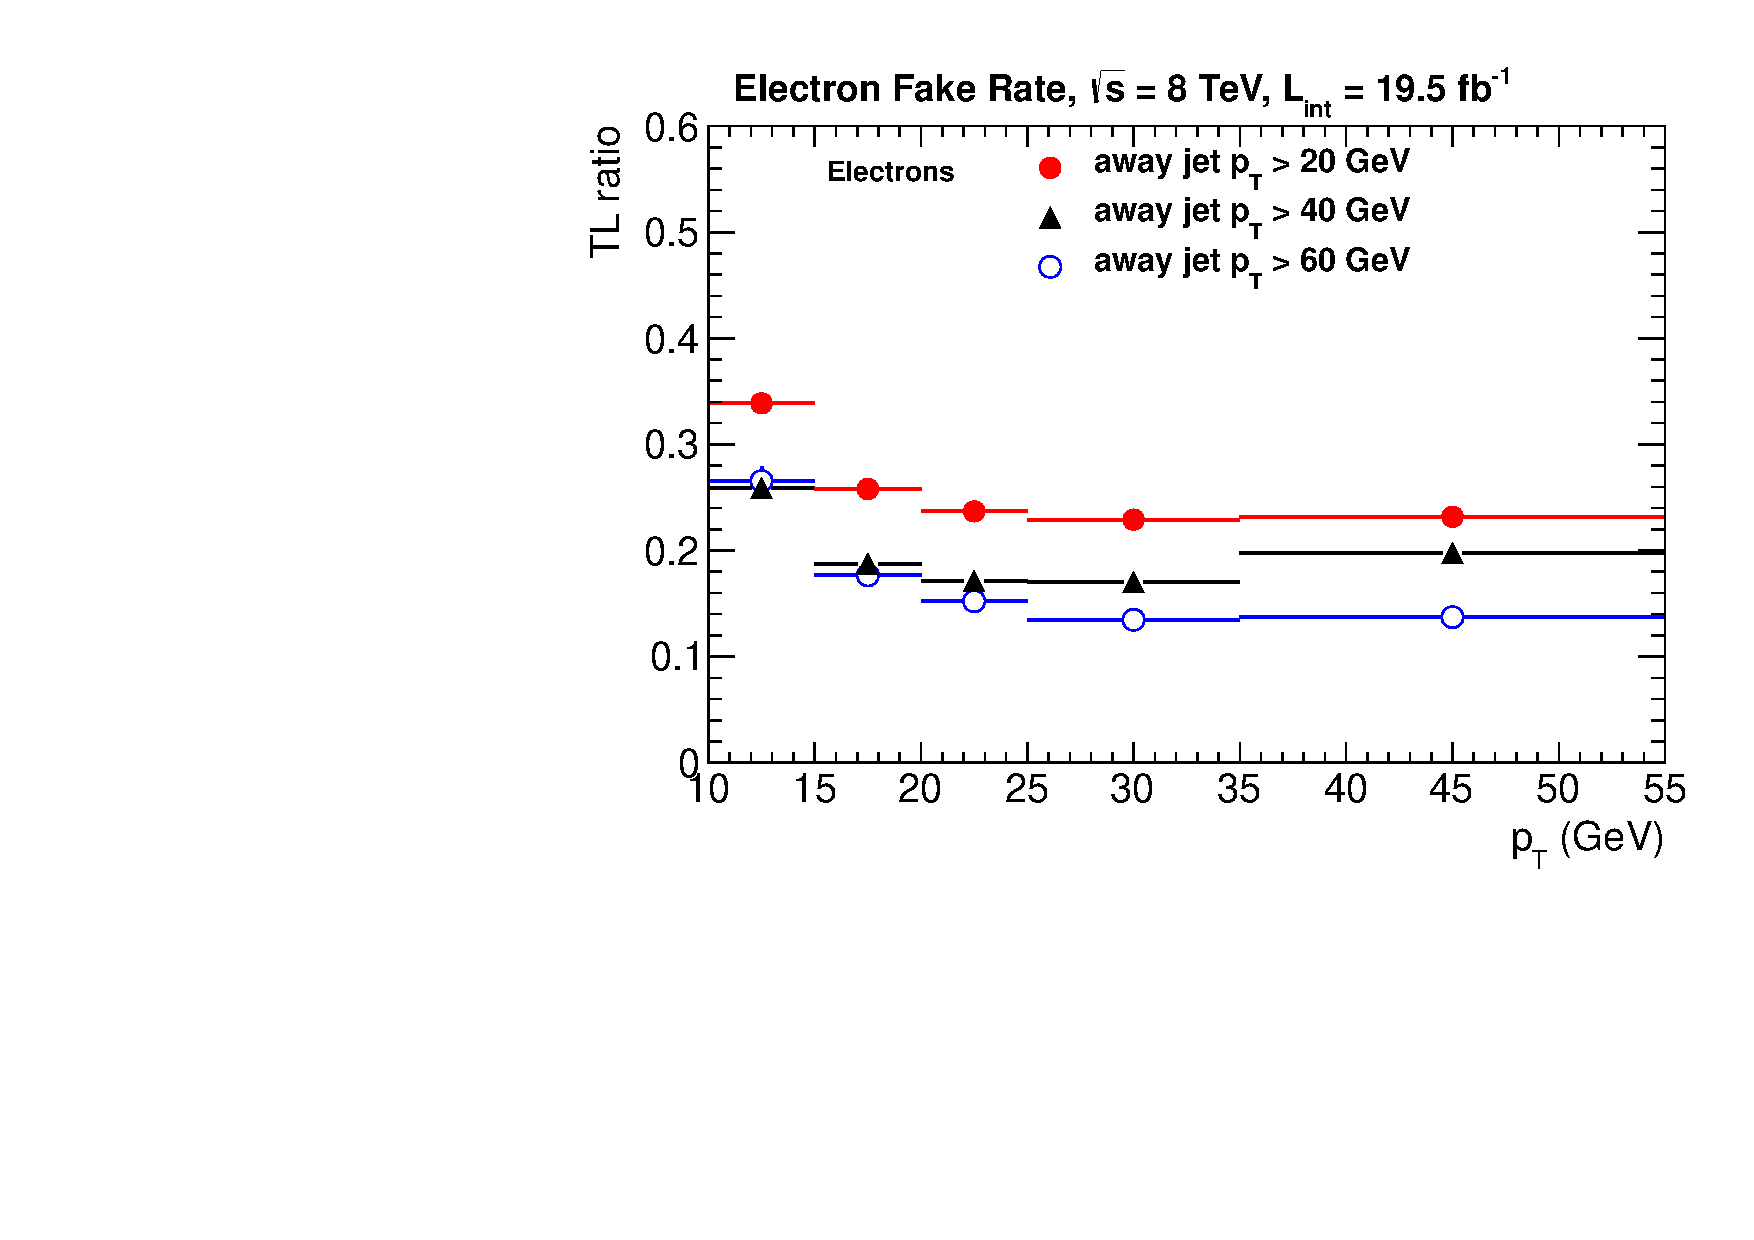
\includegraphics[width=0.48\textwidth]{p_elfr_vs_pt}
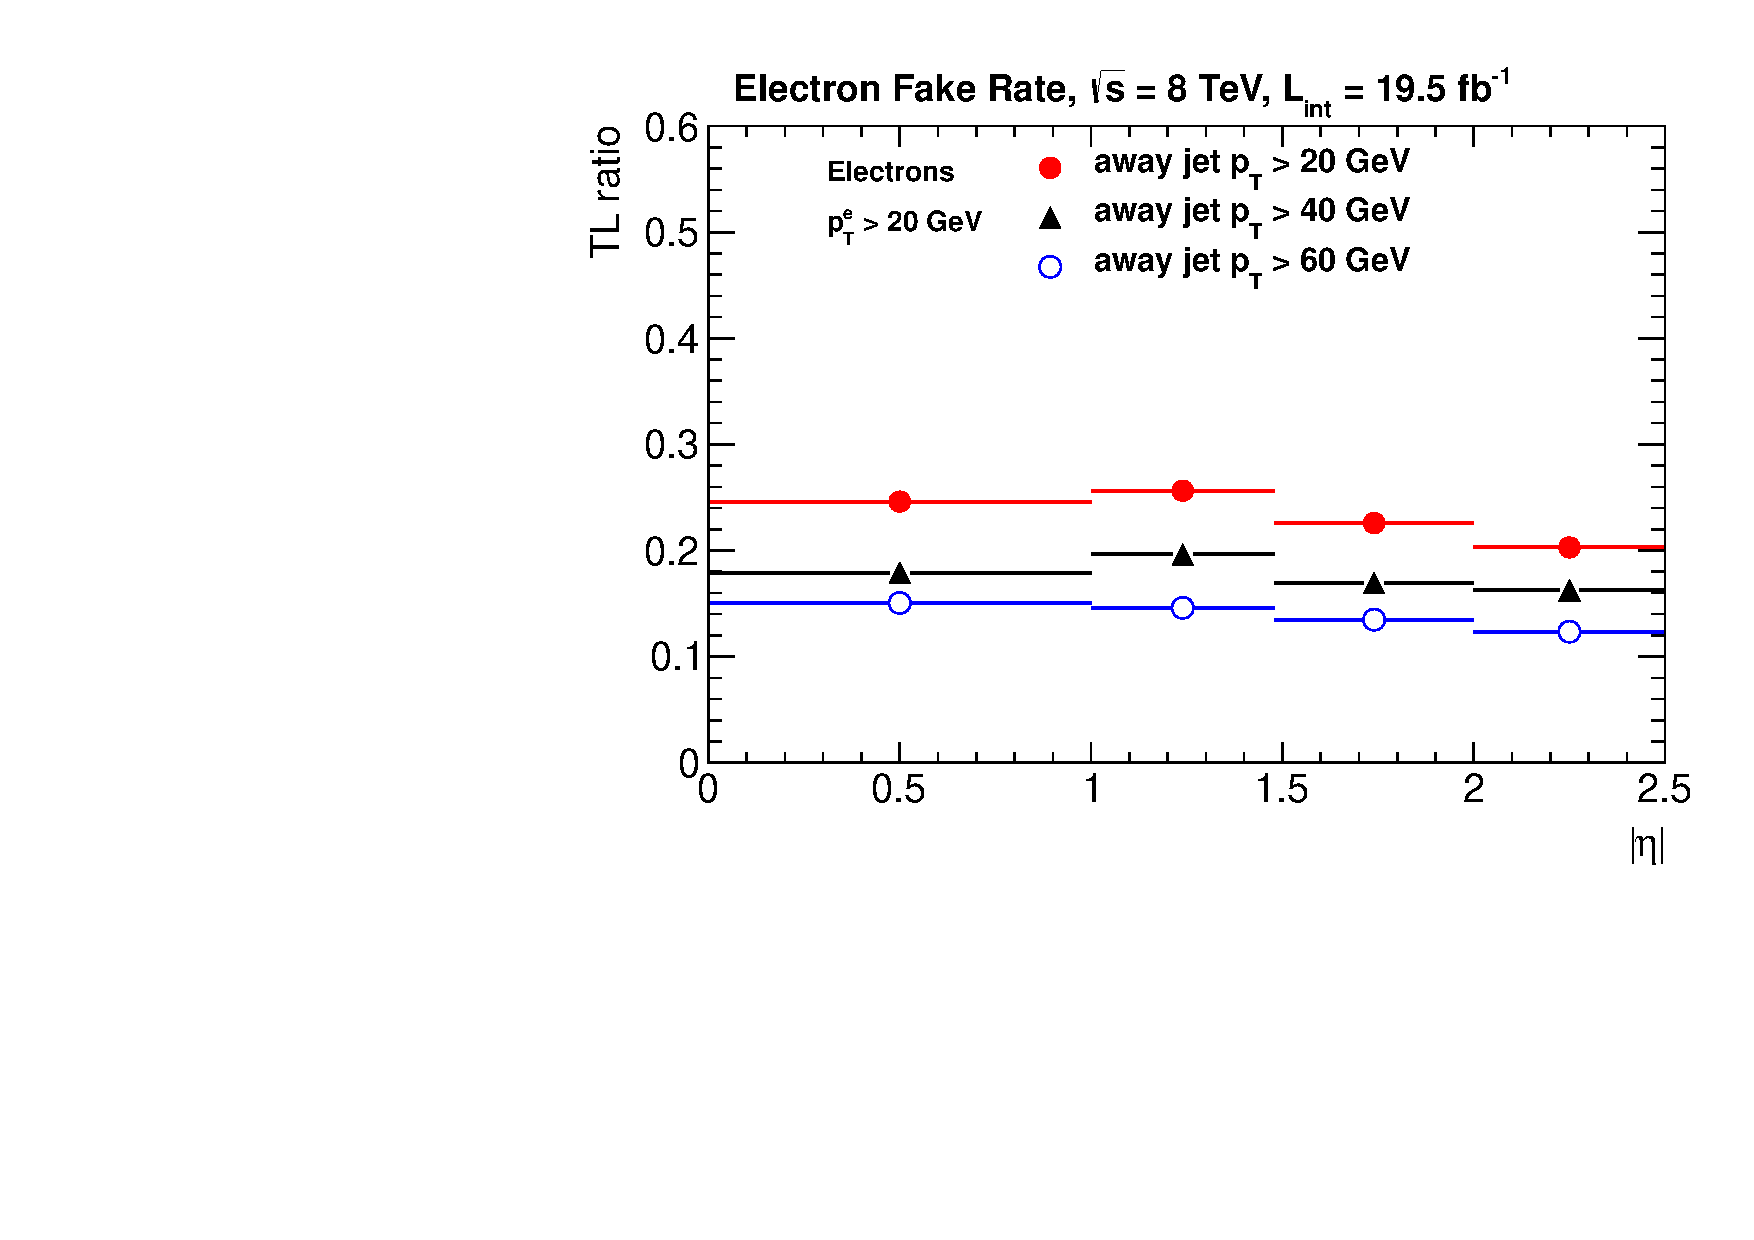
\includegraphics[width=0.48\textwidth]{p_elfr_vs_eta}
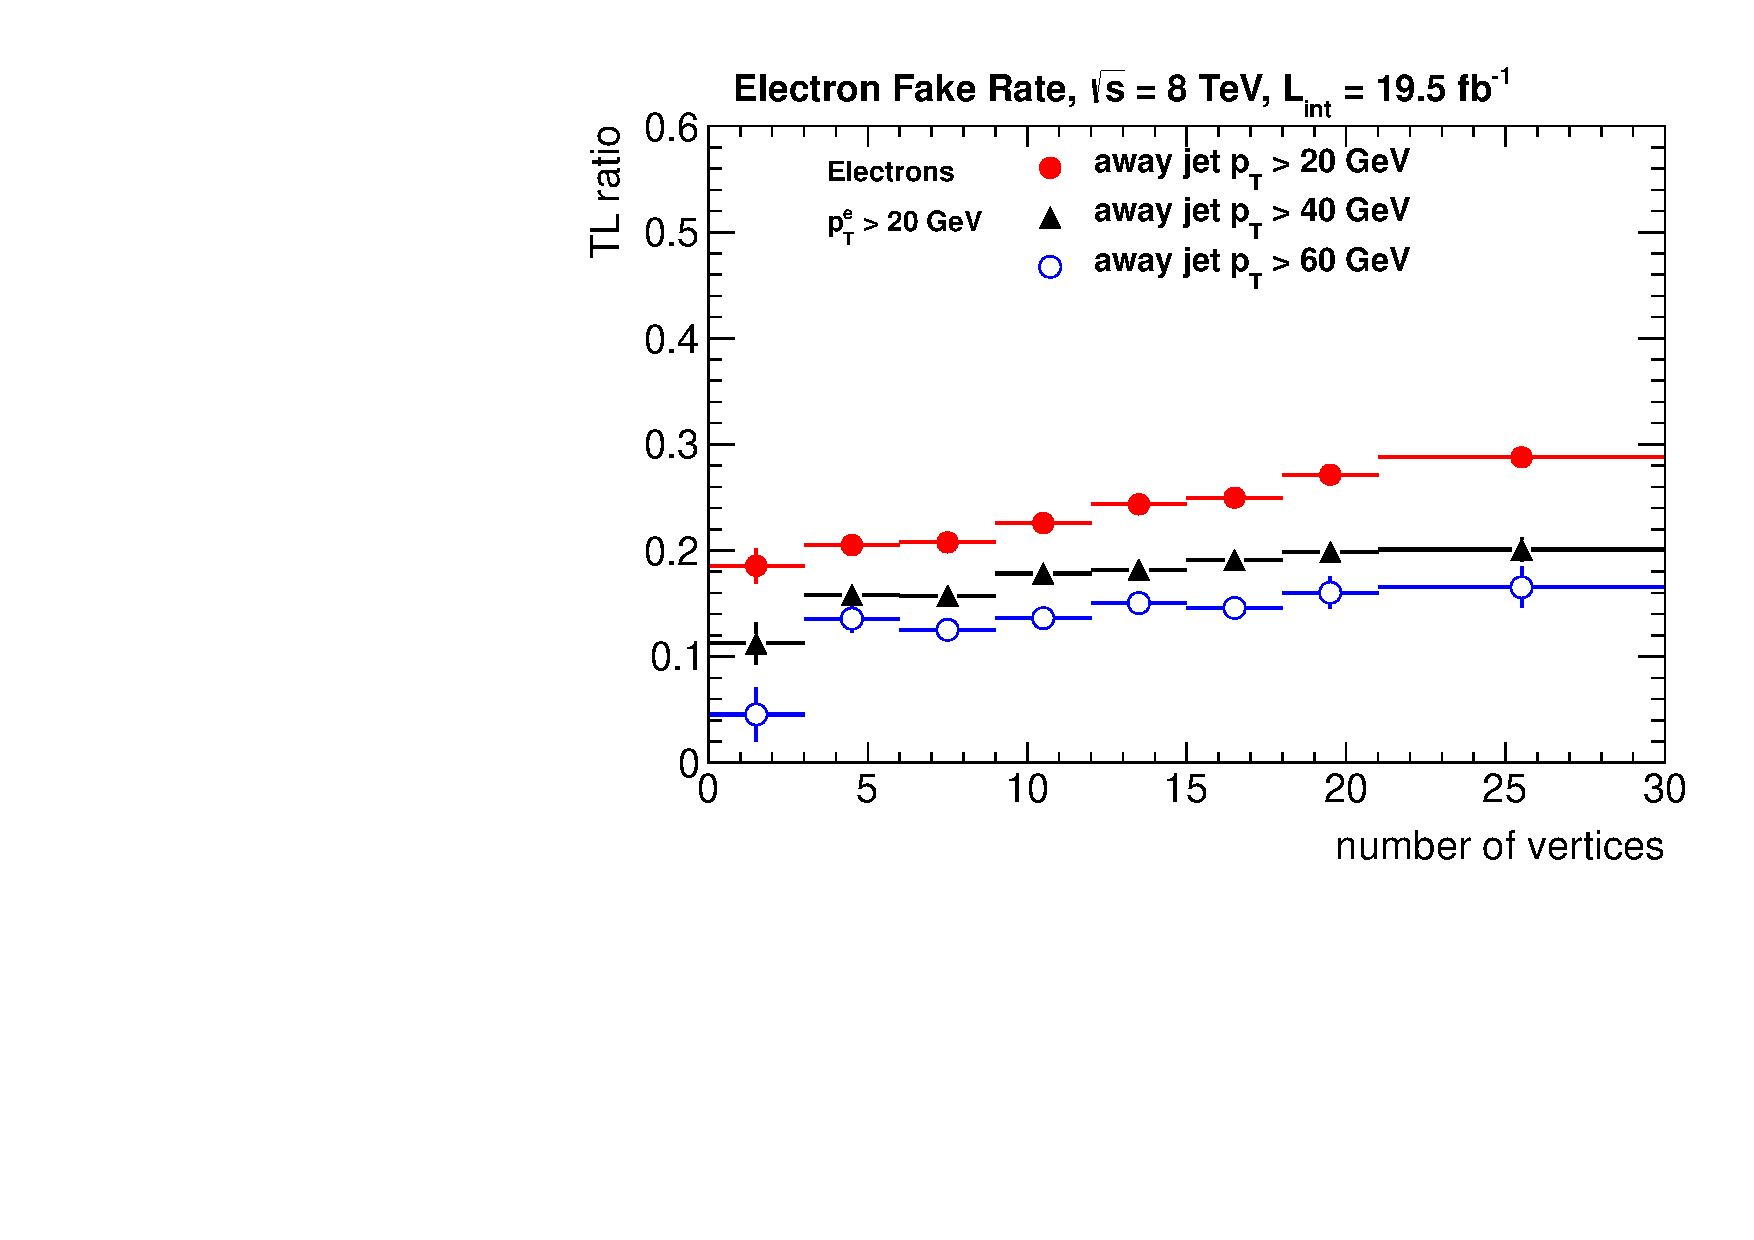
\includegraphics[width=0.48\textwidth]{p_elfr_vs_nvtxs}
\caption[Electron Fake Rate vs \pt, \aeta, and number of vertices for different away jet \pt requirements (with online isolation requirement)]
{\label{fig:bkgd_fakes_fr_elfr}
Projection of the electron fake rate in data vs \aeta, \pt, and \nvtx for
different away jet \pt requirements. The away jet is a corrected particle
flow jet and is required to be $\DR > 0.1$ away from the electron candidate.
The electron fake rate is measured using triggers with an online isolation
requirement.
}
\end{center}
\end{figure}
% --------------------------------------------------------------------------- %

% --------------------------------------------------------------------------- %
\begin{figure}[!hbt]
\begin{center}
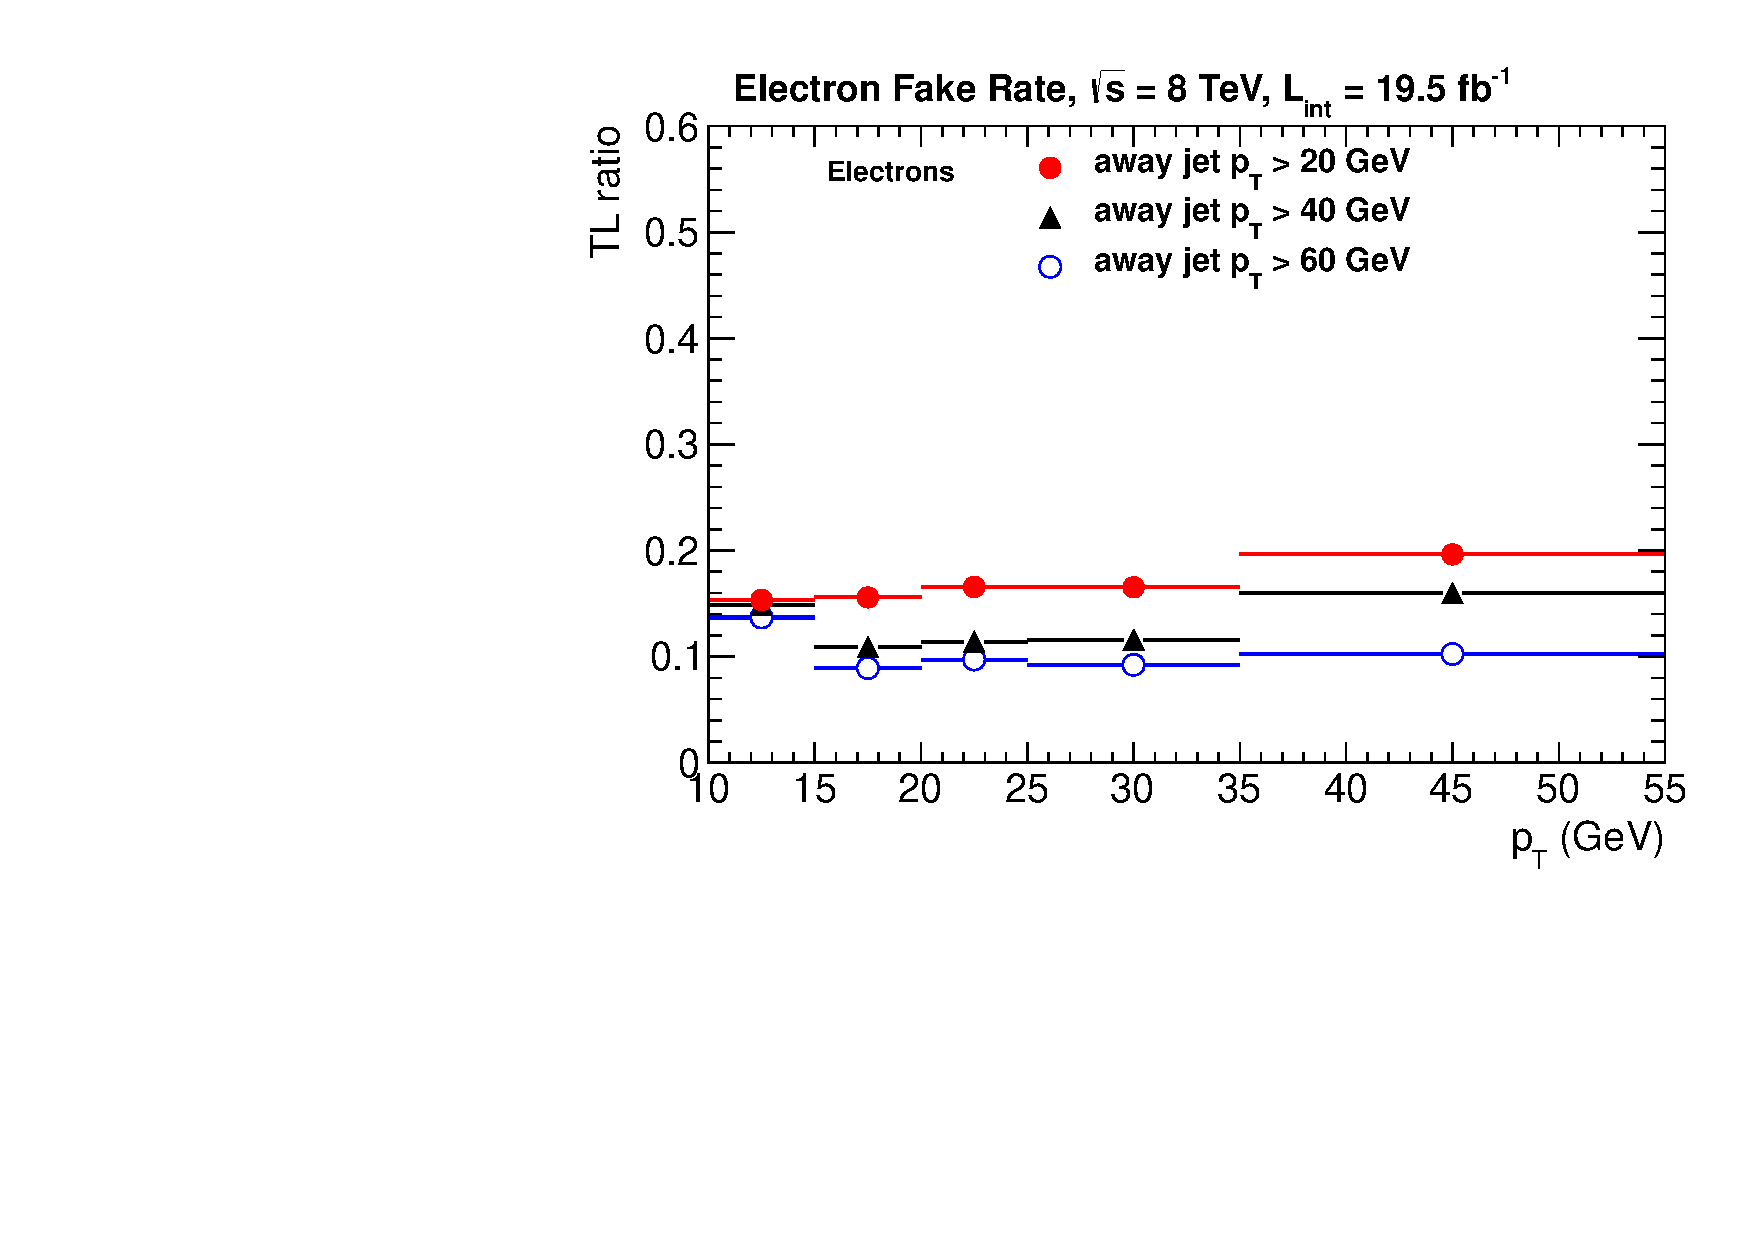
\includegraphics[width=0.48\textwidth]{p_elfr_trig_noiso_vs_pt}
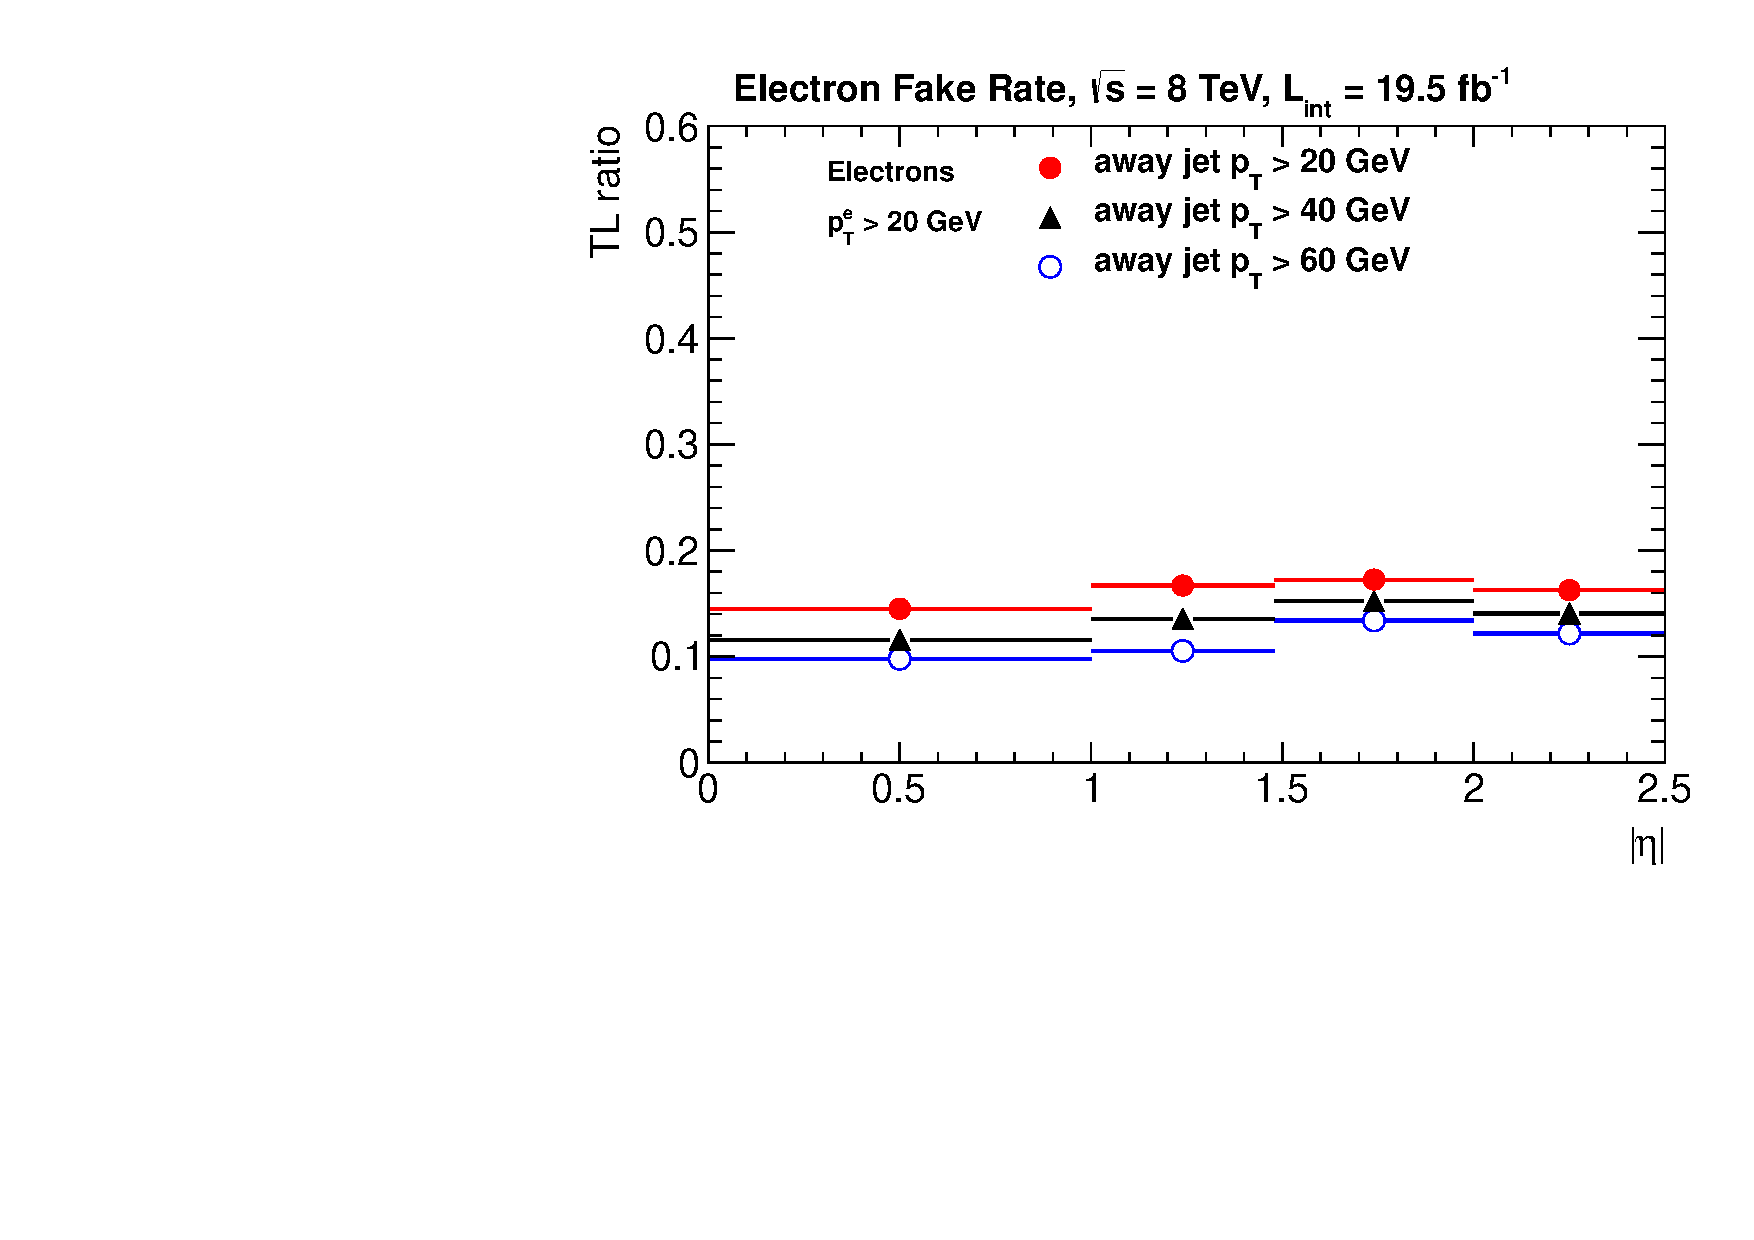
\includegraphics[width=0.48\textwidth]{p_elfr_trig_noiso_vs_eta}
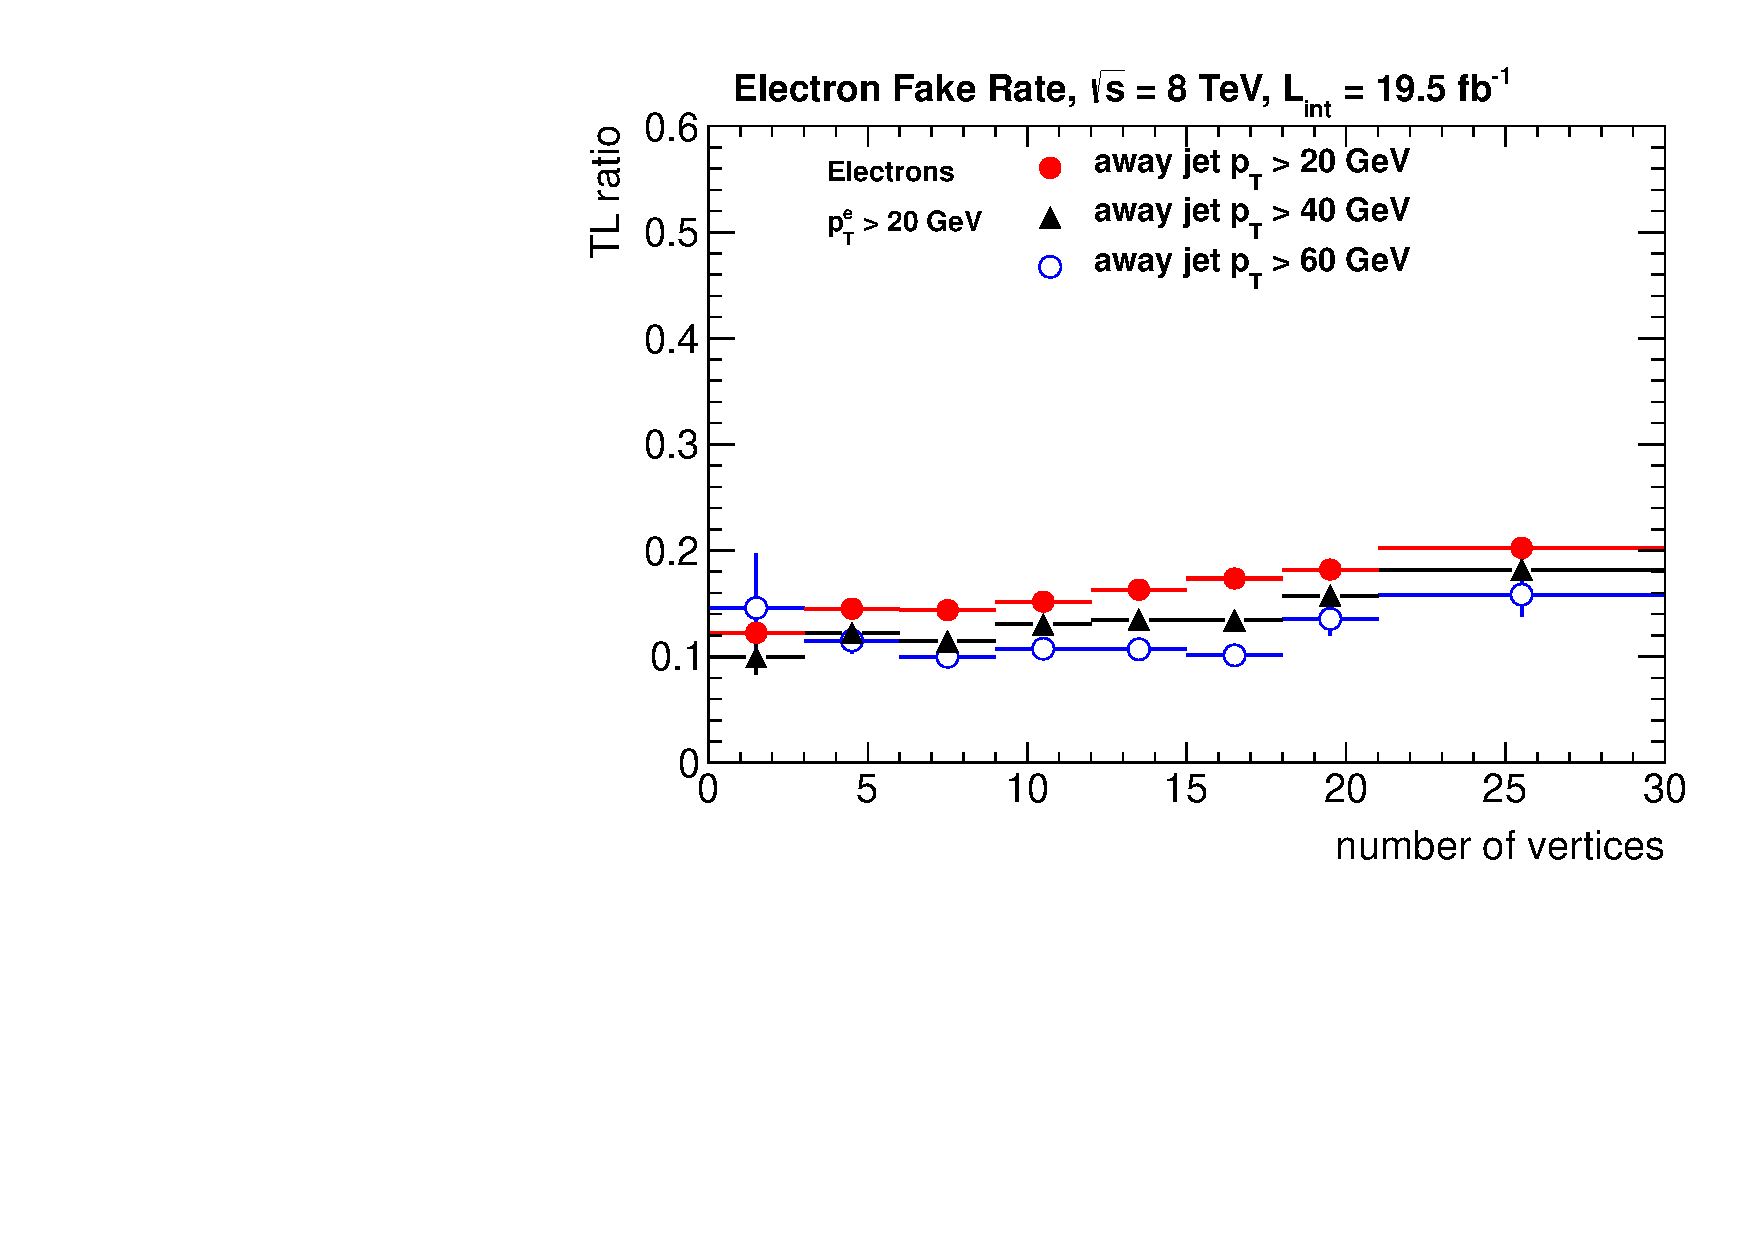
\includegraphics[width=0.48\textwidth]{p_elfr_trig_noiso_vs_nvtxs}
\caption[Electron Fake Rate vs \pt, \aeta, and number of vertices for different away jet \pt requirements (no online isolation requirement)]
{\label{fig:bkgd_fakes_fr_elfr_noiso}
Projection of the electron fake rate in data vs \aeta, \pt, and \nvtx for
different away jet \pt requirements. The away jet is a corrected particle
flow jet and is required to be $\DR > 0.1$ away from the electron candidate.
The electron fake rate is measured using triggers without an online isolation
requirement.
}
\end{center}
\end{figure}
% --------------------------------------------------------------------------- %

% --------------------------------------------------------------------------- %
\subsubsection{Fake Rate Closure Tests}
\label {sec:bkgd_fakes_frstudy_closure}
% --------------------------------------------------------------------------- %

We test that the fake rates measured in QCD are applicable to the dilepton
samples by performing a closure test on a simulated \ttbar and \Wj sample. The
closure test uses QCD MC to derive the fake rate itself and applied events
selected from \ttbar and \Wj MC sample. See Table~\ref{tab:bkgd_fakes_mc}
for the MC samples used for this test. Other dilepton processes with fakes,
such as QCD with two fakes, are expected to contribute negligibly to the events
selected in this analysis. First we describe the results of the closure test
using \ttbar and \Wj events with the QCD derived fake rate. The following selections
are applied to events entering the \ttbar and \Wj closure tests:
% --------------------------------------------------------------------------- %
\begin{enumerate}
\item Select events that pass the baseline selections (SR0, SR10, SR20). For
\Wj, the statistics was too low so only the SR0 is considered.
\item Require at truth level that for \ttbar events, the top-quark pairs decay
semi-leptonically (i.e. one $\Wlnu$ and the other $\Wqq$).
\item Require that one lepton (real) is matched to the leptonic W decay and
the other (fake) lepton is not matched to the leptonic W decay and passes the
denominator but {\bf not} the full lepton selections.  This is the FO count.
\item Scale the FO count by $\epsilon_{FR}/(1-\epsilon_{FR})$ where
$\epsilon_{FR}$ is the QCD MC derived fake rate as a function of the fake
lepton \pt~and \aeta\ -- this is the prediction of the number of fakes passing
the full lepton selections.
\item Require that one lepton (real) is matched to the leptonic W decay and the
other (fake) lepton is not matched to the leptonic W decay and passes the full
lepton selections -- this is the observed number of fake events.
\item Compare the predicted and observed number of fake events.
\end{enumerate}
% --------------------------------------------------------------------------- %
% The number of events with fake leptons in \ttbar events is consistently
% overestimated for both electrons and muons by as much as 70\%. The observations
% are consistent with studies performed during previous version of this analysis
% ~\cite{an_ss2011,an_ssb2011}.

Table~\ref{tab:bkgd_fakes_closure} shows the results of the closure test.
As in past iterations of this analysis, there is an over-prediction in
the \ttbar~MC~\cite{sspaper2010,sspaper2011}. The systematic uncertainty
of $\pm50\%$ per fake lepton is estimated for the fake rate method. Our
understanding of the these results is that the main underlying cause
is the dependence of the fake rate on the parent parton momentum. The
momentum spectrum of partons from ISR/FSR differs from that of the b-jets
or light-flavor-quark jets (\Wqq) arising from $t\to W b$ decays. The
mix of the spectra varies, but the range of the fake rate variation can
be tested in data QCD used to measure the fake rate by applying varying
threshold to the away jet as illustrated in Fig.~\ref{fig:bkgd_fakes_fr_mufr}
and~\ref{fig:bkgd_fakes_fr_elfr_noiso}.

We compute the contributions from double-fake and single-fake events separately
and based on the results of the closure test, we assign a 50\% systematic
uncertainty on the combined estimate.

% --------------------------------------------------------------------------- %
\subsubsection{Contamination from Signal Events}
\label {sec:bkgd_fakes_sc}
% --------------------------------------------------------------------------- %

Signal contamination enters when there is a significant source of two ``real''
leptons, with one or both failing the numerator selections, but passing the
denominator cuts and comprising a significant fraction of the total number of
single fake or double fake counts. An additional simulation based correction
is applied where simulated truth information is used to select events with
two real same-sign dileptons failing the numerator selections but passing the
denominator selection. These datasets correspond to the rare SM samples discussed
in Section~\ref{sec:ss_rare}. These events are weighted using the same fake rate
as we apply to data and then subtracted from the data driven prediction for
fake events. This corrected fake prediction is then used in the analysis.

% --------------------------------------------------------------------------- %
\begin{table}[!htb]
\begin{center}
\caption[Fake rate closure tests on \ttbar and \Wj events from simulation applied to a fake derived from QCD simulation]
{\label{tab:bkgd_fakes_closure}
Fake rate closure tests on \ttbar and \Wj events from simulation applied to a
fake derived from QCD simulation. The \ttbar closure test shows results for
the baseline search regions with exactly zero, exactly one and at least two
\bjs (SR0, SR10, SR20). Due to limited statistics, the \Wj closure test is only
performed on the baseline search region with a \bj veto applied (SR0).
``p'' and ``o'' refer to the predicted and the observed counts, respectively.
}
\end{center}
\resizebox{0.8\textwidth}{!}{\begin{minipage}{\textwidth}
\begin{tabular}{l|c|l|cccc}
\hline\hline
Sample                   & search region         & result   & \ee                 & \mm                & \em                  & $\ll$                \\ \hline
\multirow{12}{*}{\ttbar} & \multirow{4}{*}{SR0}  & pred     & 756.8 $\pm$ 194.8   & 830.9 $\pm$ 13.0   & 1592.7 $\pm$ 230.0   & 3180.5 $\pm$ 301.6   \\
                         &                       & obs      & 339                 & 318                & 656                  & 1313                 \\
                         &                       & pred/obs & 2.23 $\pm$ 0.59     & 2.61 $\pm$ 0.15    & 2.43 $\pm$ 0.36      & 2.42 $\pm$ 0.24      \\
                         &                       & (p-o)/p  & 0.55 $\pm$ 0.12     & 0.62 $\pm$ 0.02    & 0.59 $\pm$ 0.06      & 0.59 $\pm$ 0.04      \\ \cline{2-7}
                         & \multirow{4}{*}{SR10} & pred     & 381.3  $\pm$ 99.1   & 420.3  $\pm$ 7.9   & 804.4  $\pm$ 116.3   & 1606.0  $\pm$ 153.0  \\
                         &                       & obs      & 167                 & 177                & 354                  & 698                  \\
                         &                       & pred/obs & 2.28 $\pm$ 0.62     & 2.37 $\pm$ 0.18    & 2.27 $\pm$ 0.35      & 2.30 $\pm$ 0.24      \\
                         &                       & (p-o)/p  & 0.56 $\pm$ 0.12     & 0.58 $\pm$ 0.03    & 0.56 $\pm$ 0.07      & 0.57 $\pm$ 0.04      \\ \cline{2-7}
                         & \multirow{4}{*}{SR20} & pred     & 59.0  $\pm$ 14.9    & 45.3  $\pm$ 2.1    & 99.0  $\pm$ 13.7     & 203.4  $\pm$ 20.3    \\
                         &                       & obs      & 34                  & 23                 & 53                   & 110                  \\
                         &                       & pred/obs & 1.74 $\pm$ 0.53     & 1.97 $\pm$ 0.42    & 1.87 $\pm$ 0.36      & 1.85 $\pm$ 0.26      \\
                         &                       & (p-o)/p  & 0.42 $\pm$ 0.18     & 0.49 $\pm$ 0.11    & 0.46 $\pm$ 0.10      & 0.46 $\pm$ 0.07      \\ \hline
\multirow{4}{*}{\Wj}     & \multirow{4}{*}{SR0}  & pred     & 23.7  $\pm$ 5.9     & 4.5  $\pm$ 0.7     & 33.7  $\pm$ 7.3      & 61.9  $\pm$ 9.4      \\
                         &                       & obs      & 29                  & 4                  & 21                   & 54                   \\
                         &                       & pred/obs & 0.82 $\pm$ 0.25     & 1.13 $\pm$ 0.59    & 1.60 $\pm$ 0.49      & 1.15 $\pm$ 0.23      \\
                         &                       & (p-o)/p  & -0.22 $\pm$ 0.38    & 0.12 $\pm$ 0.46    & 0.38 $\pm$ 0.19      & 0.13 $\pm$ 0.18      \\
\hline\hline
\end{tabular}
\end{minipage}
}
\end{table}
% --------------------------------------------------------------------------- %

% --------------------------------------------------------------------------- %
% --------------------------------------------------------------------------- %
\section{Estimation of the Charge Mis-measurement Rate}
\label {sec:bkgd_flips}
% --------------------------------------------------------------------------- %
% --------------------------------------------------------------------------- %
As discussed in the Section~\ref{sec:ss_bkgd_flips} and the beginning of this
chapter, a possible source of background is lepton charge mis-measurement. As
with the fake leptons from the previous section, this may not be well modeled
by simulation, so we use a data-driven method to estimate this background.

We define a charge flip as an electron whose charge is mis-reconstructed.
We do not consider muons, as we have found previously that muon charge
flips are several orders of magnitude smaller than electron charge
flips~\cite{an_ss2010}. Further, it is difficult to correctly reconstruct
the muon \pt while incorrectly reconstructing the charge, as both come from
the track (this effect is not present in electrons since the electron \pt is
determined by the ECAL).

We expect the charge flip rate to depend on \pt and \aeta. Events with a higher
\pt will have a straighter track, and with less curvature, the charge will be
more difficult to measure. Similarly, bremsstrahlung photons in events with
higher \aeta~will be more likely to convert, since there is more material at
higher \aeta.
 
It is difficult to find a charge flip enriched data sample with kinematics
similar to our search regions. Z events give the most charge flips, but
have a very limited \pt distribution. We therefore choose to measure
the flip rate in simulation, and to test the flip rate on data. We
choose a combination of Drell-Yan and \ttbar simulated events because
these samples have good statistics and a reasonable range of \pt, see
Figure~\ref{fig:bkgd_flips_vs_pt}.

% --------------------------------------------------------------------------- %
\begin{figure}[!hbt]
\begin{center}
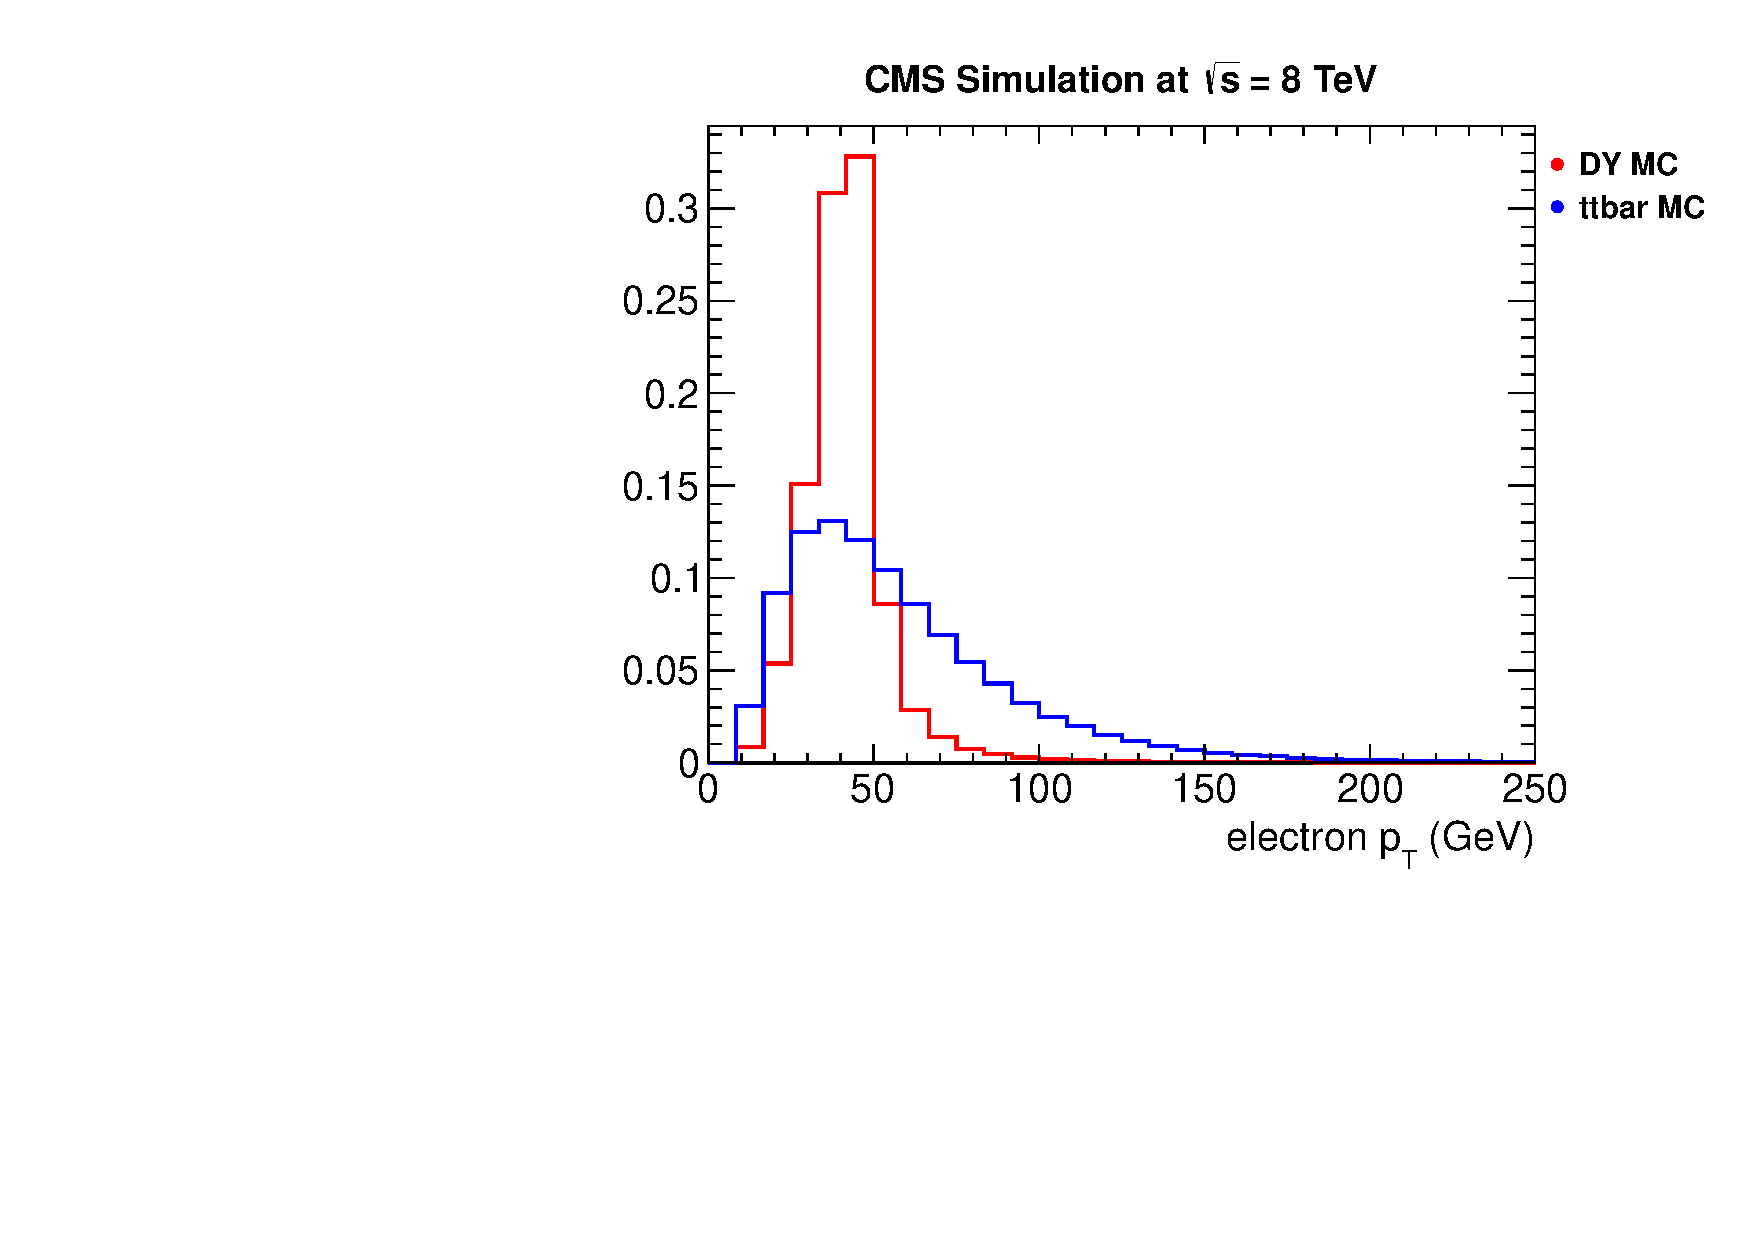
\includegraphics[width=0.8\textwidth]{p_flips_vs_pt}
\caption[The \pt distribution for electrons that pass the analysis selections]
{\label{fig:bkgd_flips_vs_pt}
The \pt distribution for electrons that pass the selections from
Section~\ref{sec:evtsel_el} for Drell-Yan and \ttbar simulated events.
}
\end{center}
\end{figure}

% --------------------------------------------------------------------------- %
We calculate the flip rate as a fraction. The denominator is the
number of electrons that pass the full selection requirements (see
Section~\ref{sec:evtsel_el}). The numerator is the number of denominator
electrons with an incorrectly reconstructed charge sign according to truth
information from the simulation. We further calculate this in bins of \pt and
\aeta. The result is shown in table \ref{tab:bkgd_flips_rate}. Notice that the
flip rate has a very significant dependence on both \pt and \aeta.
% --------------------------------------------------------------------------- %
\begin{table}[hbt!]
\begin{center}
\caption[Electron charge-flip rate as a function of \pt and \aeta]
{\label{tab:bkgd_flips_rate}
Electron charge-flip rate as a function of \pt and \aeta.
}
\end{center}
\resizebox{0.55\textwidth}{!}{\begin{minipage}{\textwidth}
\begin{tabular}{c|ccccc}
\hline\hline
\backslashbox{$|\eta|$}{$p_T$} & 0-20 \GeV                         & 20-40 \GeV                        & 40-60 \GeV                        & 60-80 \GeV                        & 80-200 \GeV                       \\ \hline
0.0-1.0                        & $2.52\ten{-05} \pm 2.52\ten{-05}$ & $3.44\ten{-05} \pm 6.18\ten{-06}$ & $2.06\ten{-05} \pm 4.38\ten{-06}$ & $1.03\ten{-04} \pm 3.27\ten{-05}$ & $9.16\ten{-05} \pm 4.58\ten{-05}$ \\
1.0-2.0                        & $1.67\ten{-04} \pm 6.29\ten{-05}$ & $1.81\ten{-04} \pm 1.82\ten{-05}$ & $2.16\ten{-04} \pm 1.94\ten{-05}$ & $5.31\ten{-04} \pm 1.00\ten{-04}$ & $9.87\ten{-04} \pm 2.06\ten{-04}$ \\
2.0-2.4                        & $0.00\ten{+00} \pm 4.52\ten{-05}$ & $2.96\ten{-04} \pm 4.52\ten{-05}$ & $3.96\ten{-04} \pm 5.49\ten{-05}$ & $1.34\ten{-03} \pm 3.34\ten{-04}$ & $8.79\ten{-04} \pm 4.39\ten{-04}$ \\
\hline\hline
\end{tabular}
\end{minipage}
}
\end{table}

% --------------------------------------------------------------------------- %
We validate by making a prediction and an observation using the flip rate
applied to data. We start by selecting electron pairs that pass the analysis
\pt, \aeta, and electron ID and isolation requirements which are listed
in Section \ref{sec:evtsel_el}. Also, these events must pass the dilepton
trigger (for data) from Section~\ref{sec:evtsel_trig}, and the dilepton
invariant mass should be between 76 \GeV and 106 \GeV for exactly one pair of
electrons. The observation is then simply the number of same sign dilepton
events occurring in the above dilepton selection. For the prediction, the flip
rate (which was derived in simulation) is applied to this selection: we select the
opposite-sign dielectron events in the sample, weighting each one with a factor
of
% --------------------------------------------------------------------------- %
\[ 
\frac{\epsilon_{fl,1}}{1 - \epsilon_{fl,1}} + \frac{\epsilon_{fl,2}}{1 - \epsilon_{fl,2}}
\]
% --------------------------------------------------------------------------- %
where the flip rate for the nth electron, $\epsilon_{fl, n}$, is taken from
table \ref{tab:bkgd_flips_rate}. The denominator is necessary because we are
not summing over the same-sign dielectron pairs.
 
In data, we predict 944 same-sign events and observe 1561 events. The
invariant mass distribution for these 1561 events is shown in figure
\ref{fig:bkgd_flips_ss_mee}. However, we must investigate the possibility of
non-Z events occurring in the data sample, causing our observation to be
artificially high.
% --------------------------------------------------------------------------- %
\begin{figure}[!hbt]
\begin{center}
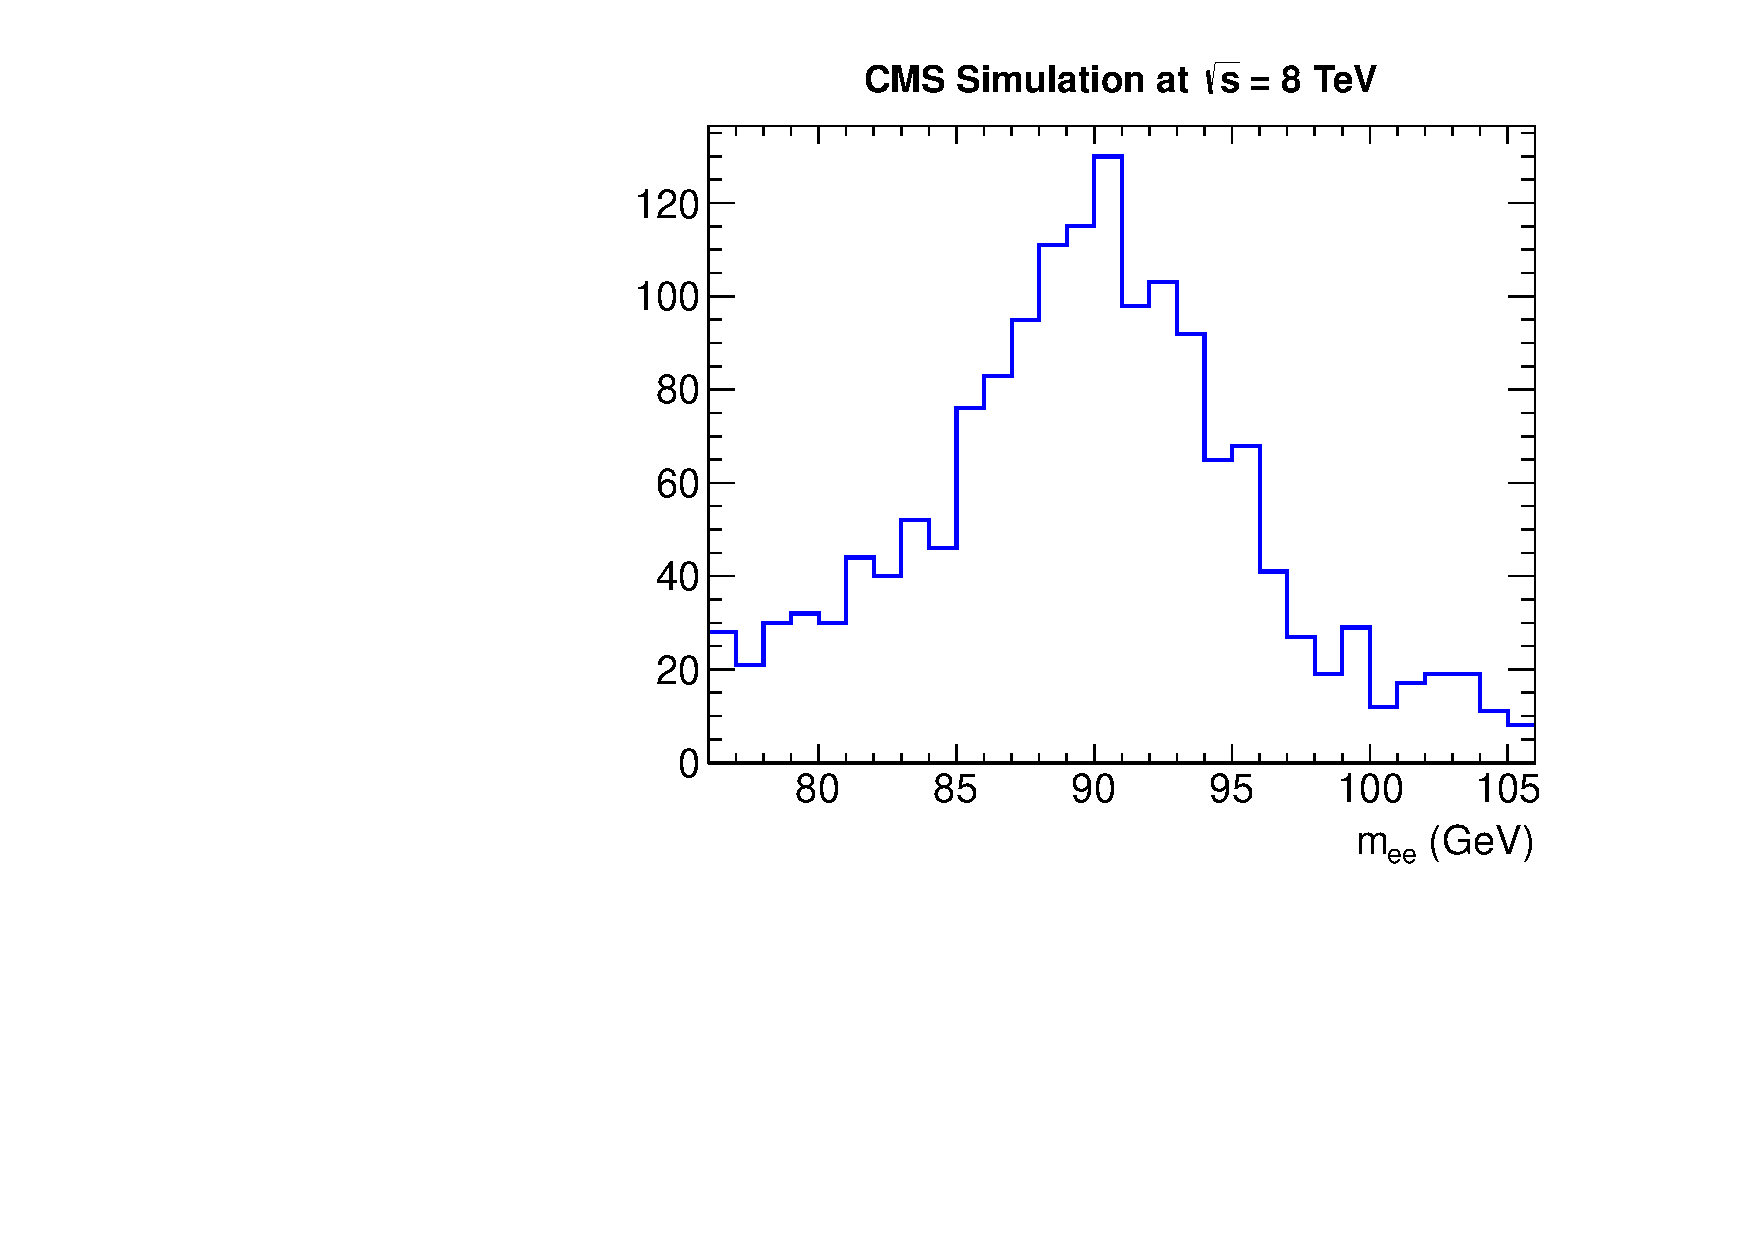
\includegraphics[width=0.8\textwidth]{p_ss_mee}
\caption[The \mee distribution for same-sign electron pairs in data]
{\label{fig:bkgd_flips_ss_mee}
The \mee distribution for same-sign electron pairs in data.
}
\end{center}
\end{figure}

% --------------------------------------------------------------------------- %
We consider the upper sidebands in the dilepton mass plot of the data charge
flips ($106\ \GeV < \mee < 121\ \GeV$). Figure \ref{fig:bkgd_flips_mee} shows
that events in this region are unlikely to be flips from high mass Zs, and
so we may assume as an approximation that everything in this region is a
contamination. Figure \ref{fig:bkgd_flips_ss_mee} shows that a significant
number of electrons are indeed predicted in this region. In order to compare
with the prediction from simulation, we subtract these events from the full
data prediction. We extrapolate from this figure that about 16\% of the
observed flips are actually contamination rather than charge flips. We use this
factor to adjust our number of observed charge flips.
% --------------------------------------------------------------------------- %
\begin{figure}[!hbt]
\begin{center}
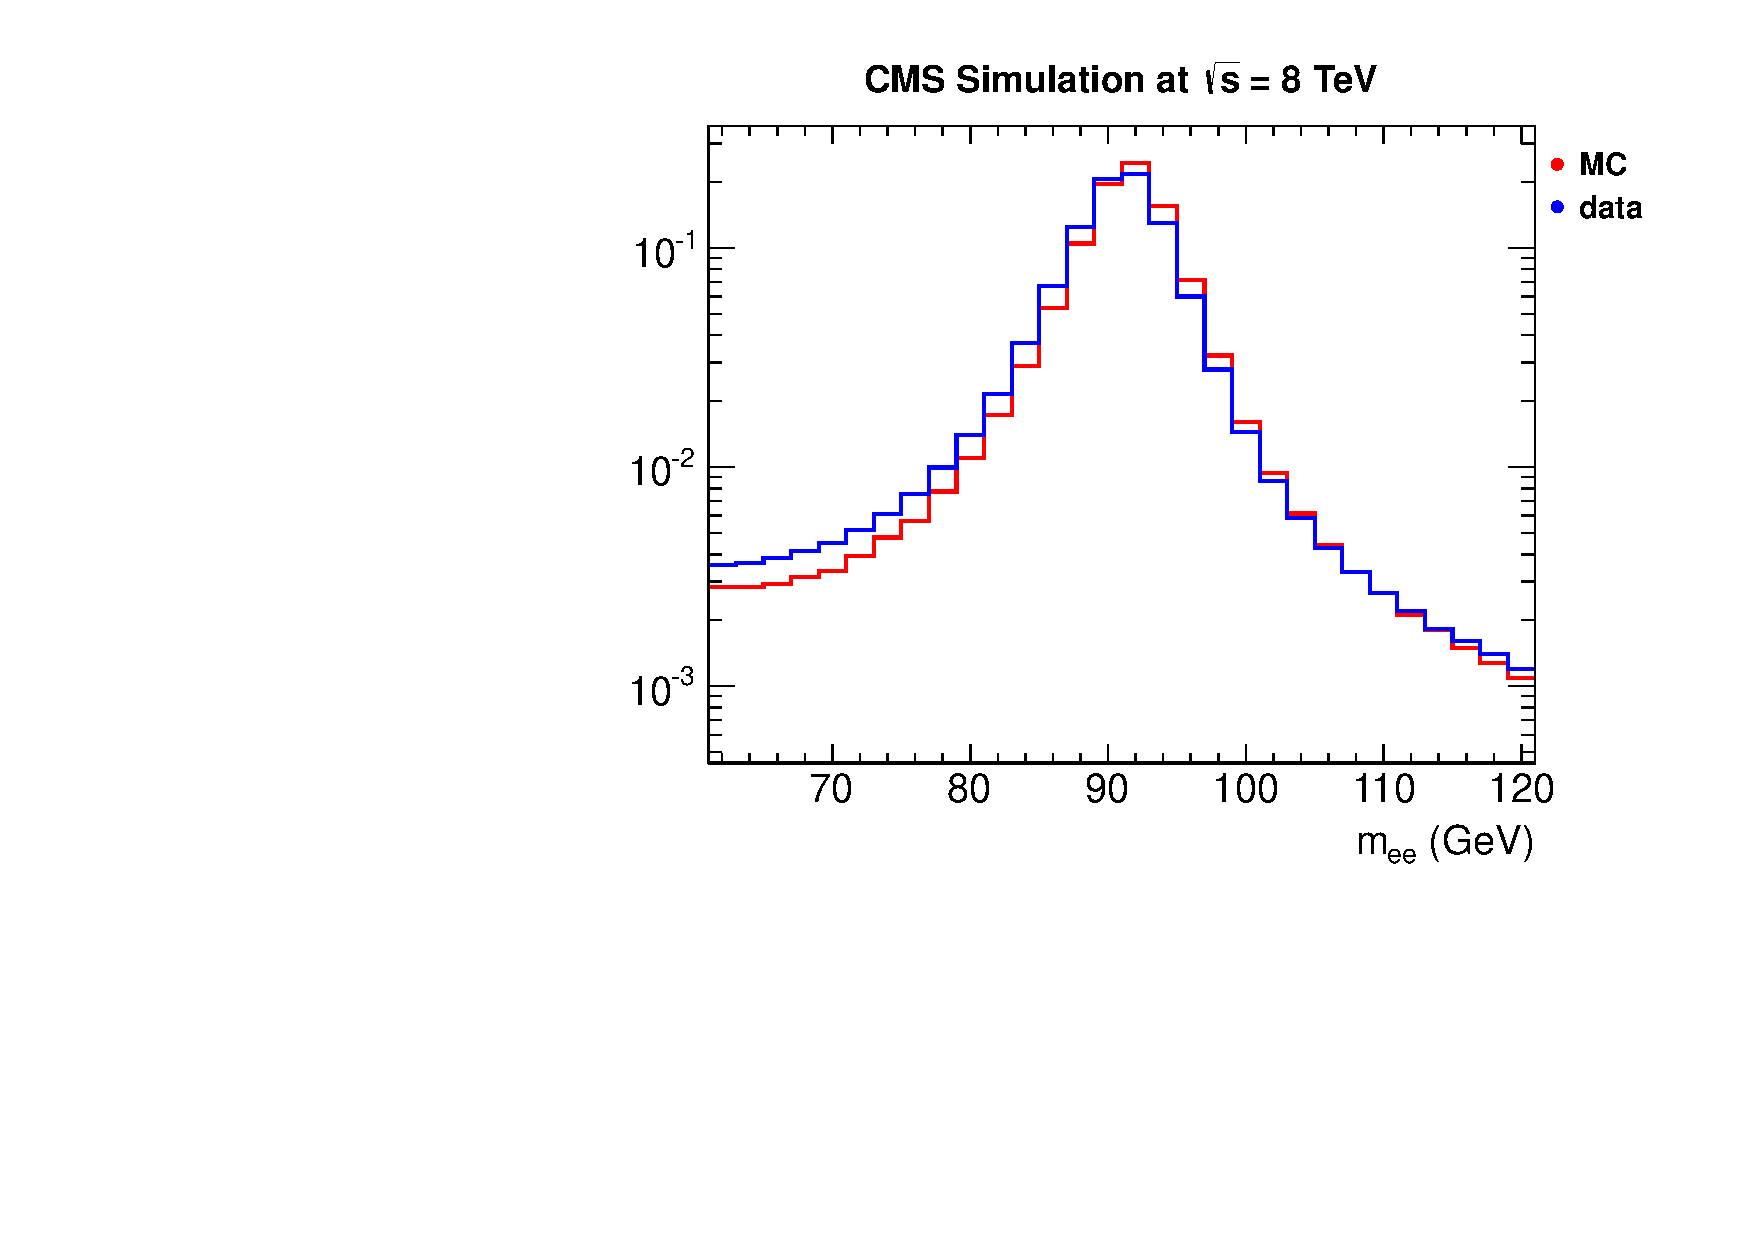
\includegraphics[width=0.8\textwidth]{p_os_mee}
\caption[The \mee distribution for opposite-sign electron pairs in data]
{\label{fig:bkgd_flips_mee}
The \mee distribution for opposite-sign electron pairs in data.
}
\end{center}
\end{figure}

% --------------------------------------------------------------------------- %
The result is that we expect 944 charge flips, and we observe 1311. We
reconcile these two differences with a scale factor:
\[ SF = \textrm{observed/predicted} = 1.39 \]
So the flip rates in Table~\ref{tab:bkgd_flips_rate}, multiplied by the scale
factor, should give a good approximation of the overall flip rate.

This remaining discrepancy, coupled with the kinematic limitation of the       
control sample, allow for considerable error in our estimation of the charge   
flip background. We therefore assign an overall systematic of $\pm\ 30\%$ to   
allow for these.                                                               

% --------------------------------------------------------------------------- %
% --------------------------------------------------------------------------- %
\section{Rare SM background estimation}
\label {sec:bkgd_rare}
% --------------------------------------------------------------------------- %
% --------------------------------------------------------------------------- %
Backgrounds arising from failures of lepton identification and electron charge
mis-reconstruction together account for 40-70\% of the estimated background in
a given search region. The remaining 30-60\% of the background is irreducible
and is taken directly from simulation. A list of the process and associated
cross sections is provided in Table~\ref{tab:evtsel_datasets_rare} and repeated
here for convenience. Note that we neglect contributions from $W\gamma^{*}
\rightarrow \ell \nu ee$ because the simulated dataset was known to be faulty
and this process contributes less than a percent to the irreducible background
total.
% --------------------------------------------------------------------------- %
%\begin{landscape}
\begin{table}[!hbt]
\begin{center}
\caption[Sources of true same-sign dileptons from Standard Model processes]
{\label{tab:bkgd_datasets_mc}
Sources of true same-sign dileptons from Standard Model processes. Cross
sections are next-to-leading order. The equivalent integrated luminosity
of these simulated events is listed in the column on the far right. The
contributions from these process to the background is taken directly from
simulation.
}
\footnotesize{
    \begin{tabular}{lccc}
    \hline\hline
    Sample     & Cross Section (pb) & Equivalent Luminosity (\fbinv) \\ \hline
    \ttZ       & 0.208              & 1021                           \\
    \ttW       & 0.232              & 845                            \\
    \ttWW      & 0.00204            & 106931                         \\
    \ttG       & 2.17               & 33                             \\
    \tbZ       & 0.0114             & 13026                          \\
    \ZZZ       & 0.00554            & 40692                          \\
    \WWW       & 0.0822             & 2737                           \\
    \WWG       & 0.528              & 407                            \\
    \WZZ       & 0.0192             & 12946                          \\
    \WWZ       & 0.0580             & 3832                           \\
    \ZZ        & 0.177              & 27177                          \\
    \WZ        & 1.058              & 1908                           \\
    \qqWmWm    & 0.0889             & 1084                           \\
    \qqWpWp    & 0.248              & 402                            \\
    \WWdps     & 0.588              & 1418                           \\
    \Wgsmm     & 1.91               & 156                            \\
    \Wgstt     & 0.336              & 148                            \\
    \HToWW     & 0.260              & 769                            \\
    \HToZZ     & 0.0320             & 15652                          \\
    \HToTauTau & 0.0177             & 5478                           \\
    \hline\hline
    \end{tabular}
}
\end{center}
\end{table}

% --------------------------------------------------------------------------- %
Most of the background involving rare SM process have never been measured
before. The cross sections used for these processes are next-to-leading (NLO)
order and are used to normalize the rare predictions. The cross section values
used for the most relevant processes, \ttW and \ttZ, are 232 \fb and 208 \fb,
respectively~\cite{ttw,ttz}. The systematic uncertainty for the rare SM
backgrounds accounts for the theoretical uncertainty on the cross sections as
well as for the ratio between LO (as in simulation) and NLO cross-sections being
non-uniform as a function of jet multiplicity, \Ht and \met. Due to this, a
50\% systematic uncertainty for the prediction from these rare SM processes is
assigned.
